% !TeX encoding = UTF-8
% !TeX spellcheck = de_DE
%%%%%%%%%%%%%%%%%%%%%%%%%%%%%%%%%%%%%%%%%
% Arsclassica Article
% LaTeX Template
% Version 1.1 (10/6/14)
%
% This template has been downloaded from:
% http://www.LaTeXTemplates.com
%
% Original author:
% Lorenzo Pantieri (http://www.lorenzopantieri.net) with extensive modifications by:
% Vel (vel@latextemplates.com)
%
% License:
% CC BY-NC-SA 3.0 (http://creativecommons.org/licenses/by-nc-sa/3.0/)
% 
%%%%%%%%%%%%%%%%%%%%%%%%%%%%%%%%%%%%%%%%%

%----------------------------------------------------------------------------------------
%	PACKAGES AND OTHER DOCUMENT CONFIGURATIONS
%----------------------------------------------------------------------------------------

\documentclass[
11pt, % Main document font size
a4paper, % Paper type, use 'letterpaper' for US Letter paper
oneside, % One page layout (no page indentation)
%twoside, % Two page layout (page indentation for binding and different headers)
pdfspacing, % Makes use of pdftex’ letter spacing capabilities via the microtype package
headinclude,
%footinclude, % Extra spacing for the header and footer
BCOR=5mm, % Binding correction
ngerman, %set document to German
bibliography=totoc,
abstract=on,
]{scrartcl}
%{scrartcl}

% !TeX root = ./mainDoc.tex

%%%%%%%%%%%%%%%%%%%%%%%%%%%%%%%%%%%%%%%%%
% Arsclassica Article
% Structure Specification File
%
% This file has been downloaded from:
% http://www.LaTeXTemplates.com
%
% Original author:
% Lorenzo Pantieri (http://www.lorenzopantieri.net) with extensive modifications by:
% Vel (vel@latextemplates.com)
%
% License:
% CC BY-NC-SA 3.0 (http://creativecommons.org/licenses/by-nc-sa/3.0/)
%
%%%%%%%%%%%%%%%%%%%%%%%%%%%%%%%%%%%%%%%%%

%----------------------------------------------------------------------------------------
%	REQUIRED PACKAGES
%----------------------------------------------------------------------------------------

\usepackage[usenames,dvipsnames]{color} % Required for specifying custom colors and referring to colors by name

\usepackage[
nochapters, % Turn off chapters since this is an article        
beramono, % Use the Bera Mono font for monospaced text (\texttt)
eulermath,% Use the Euler font for mathematics
eulerchapternumbers,
pdfspacing, % Makes use of pdftex’ letter spacing capabilities via the microtype package
dottedtoc % Dotted lines leading to the page numbers in the table of contents
]{classicthesis} % The layout is based on the Classic Thesis style


\usepackage{arsclassica} % Modifies the Classic Thesis package
%checkout https://tex.stackexchange.com/a/450098/123262 to get arsclassica working with lmodern...
%\usepackage{lmodern}	
%\titleformat{\paragraph}[runin]
%  {\normalfont\normalsize\sffamily}
%  {\textssc{\MakeTextLowercase{\theparagraph}}}%
%  {0pt}{\spacedlowsmallcaps}

\usepackage[T1]{fontenc} % Use 8-bit encoding that has 256 glyphs

\usepackage[utf8]{inputenc} % Required for including letters with accents
\usepackage{textcomp} % required for ° Symbol, https://en.wikibooks.org/wiki/LaTeX/Special_Characters#Degree_symbol_for_temperature_and_math

\usepackage{graphicx} % Required for including images
\graphicspath{{Figures/}} % Set the default folder for images

\usepackage{enumitem} % Required for manipulating the whitespace between and within lists

\usepackage{lipsum} % Used for inserting dummy 'Lorem ipsum' text into the template

\usepackage{amsmath,amssymb,amsthm} % For including math equations, theorems, symbols, etc
\numberwithin{equation}{section} %https://tex.stackexchange.com/questions/106935/how-to-include-chapter-number-in-equation-numbers
\numberwithin{figure}{section}

\usepackage{varioref} % More descriptive referencing

\usepackage{url}

%for printout, use option [hidelinks]
\usepackage{hyperref}
%for digital distribution, mark links in appropriate color
%\usepackage{hyperref}

\usepackage{afterpage} %http://blog.peschla.net/2012/11/latex-footnotes-in-captions/
\usepackage{pdflscape}

\usepackage{colortbl}
\usepackage{multirow}
\usepackage{geometry}


\usepackage[ngerman, english]{babel}

\usepackage[square,
authoryear,
%numbers,
%longnamesfirst,
]{natbib}

\usepackage{enumitem}

\usepackage{authblk}

\usepackage{relsize, etoolbox}% http://ctan.org/pkg/{relsize,etoolbox}

\AtBeginEnvironment{quote}{\smaller\fontfamily{lmss}\selectfont}% Step font down one size relative to current font.
% see http://tex.stackexchange.com/questions/25249/how-do-i-use-a-particular-font-for-a-small-section-of-text-in-my-document for fontfamilies


\usepackage{listofsymbols} % Für Symbolverzeichnis

\usepackage{nicefrac} % für schräge Brüche https://de.wikibooks.org/wiki/LaTeX-W%C3%B6rterbuch:_nicefrac

\usepackage{mdframed}

% to have a separation in the text with extra space between paragraphs and no indendation following
\newcommand*{\skippingparagraph}{\par\vspace{1.0\baselineskip}\noindent}

\newcounter{reqnum}
\newcommand{\reqP}[1]{\vspace{0pt}\noindent\textbf{Anforderung \refstepcounter{reqnum}\thereqnum:\ \label{#1}}\textbf}

\usepackage{multicol}
\usepackage{booktabs}
\usepackage{chngcntr}
\usepackage{tabularx}
\usepackage{listliketab}

%Place floats where they belong to:-) 
%see https://tex.stackexchange.com/questions/118662/use-placeins-for-subsections
\usepackage{float}
\usepackage[section]{placeins}
\makeatletter
\AtBeginDocument{%
  \expandafter\renewcommand\expandafter\subsection\expandafter{%
    \expandafter\@fb@secFB\subsection
  }%
}
\makeatother


%----------------------------------------------------------------------------------------
%	HYPERLINKS
%---------------------------------------------------------------------------------------
\definecolor{mediumviolet-red}{rgb}{0.78, 0.08, 0.52}
\hypersetup{
%	draft, % Uncomment to remove all links (useful for printing in black and white)
	colorlinks=true, breaklinks=true, bookmarks=true,bookmarksnumbered,
	urlcolor=webbrown, linkcolor=mediumviolet-red, citecolor=webgreen, % Link colors
	pdftitle={}, % PDF title
	pdfauthor={\textcopyright}, % PDF Author
	pdfsubject={}, % PDF Subject
	pdfkeywords={}, % PDF Keywords
	pdfcreator={pdfLaTeX}, % PDF Creator
	pdfproducer={LaTeX with hyperref and ClassicThesis} % PDF producer
}

%----------------------------------------------------------------------------------------
%	TODONOTES
%---------------------------------------------------------------------------------------
\let\marginpar\oldmarginpar	%as seen in https://tex.stackexchange.com/a/33429/123262
\usepackage[colorinlistoftodos]{todonotes}

\newcommand{\todoInfo}[1]{\todo[color=blue!25]{INFO: #1}}
\newcommand{\todoCite}[1]{\todo[color=green!40]{INFO: #1}}


%----------------------------------------------------------------------------------------
%	CODESNIPPETS
%---------------------------------------------------------------------------------------

%%%%%%%%%%%%%%%%%%%%%%%%%%%%%%%%%%%%%%%%%
% Code Snippet
% LaTeX Template
% Version 1.0 (14/2/13)
%
% This template has been downloaded from:
% http://www.LaTeXTemplates.com
%
% Original author:
% Velimir Gayevskiy (vel@latextemplates.com)
%
% License:
% CC BY-NC-SA 3.0 (http://creativecommons.org/licenses/by-nc-sa/3.0/)
%
%%%%%%%%%%%%%%%%%%%%%%%%%%%%%%%%%%%%%%%%%
\usepackage{listings} % Required for inserting code snippets

\definecolor{DarkGreen}{rgb}{0.0,0.4,0.0} % Comment color
\definecolor{highlight}{RGB}{255,251,204} % Code highlight color
\definecolor{DogwoodRose}{rgb}{0.84, 0.09, 0.41}
\definecolor{lemonchiffon}{rgb}{1.0, 0.98, 0.8}
\definecolor{lightgoldenrodyellow}{rgb}{0.98, 0.98, 0.82}
\definecolor{oldlace}{rgb}{0.99, 0.96, 0.9}
\definecolor{oldlavender}{rgb}{0.47, 0.41, 0.47}
\definecolor{pakistangreen}{rgb}{0.0, 0.4, 0.0}
\definecolor{ao}{rgb}{0.0, 0.0, 1.0}
\definecolor{britishracinggreen}{rgb}{0.0, 0.26, 0.15}
\definecolor{coquelicot}{rgb}{1.0, 0.22, 0.0}
\definecolor{cordovan}{rgb}{0.54, 0.25, 0.27}
\definecolor{darkcandyapplered}{rgb}{0.64, 0.0, 0.0}
\definecolor{mediumchampagne}{rgb}{0.95, 0.9, 0.67}

\lstdefinestyle{Style1}{ % Define a style for your code snippet, multiple definitions can be made if, for example, you wish to insert multiple code snippets using different programming languages into one document
	language=JavaScript, % Detects keywords, comments, strings, functions, etc for the language specified
	backgroundcolor=\color{oldlace}, % Set the background color for the snippet - useful for highlighting
	basicstyle=\smaller\smaller\ttfamily, % The default font size and style of the code
	breakatwhitespace=true, % If true, only allows line breaks at white space
	breaklines=true, % Automatic line breaking (prevents code from protruding outside the box)
	captionpos=b, % Sets the caption position: b for bottom; t for top
	commentstyle=\usefont{T1}{pcr}{m}{sl}\color{ao}\textbf, % {m}DarkGreen Style of comments within the code - dark green courier font
	deletekeywords={}, % If you want to delete any keywords from the current language separate them by commas
	%escapeinside={\%}, % This allows you to escape to LaTeX using the character in the bracket
	firstnumber=1, % Line numbers begin at line 1
	frame=single, % Frame around the code box, value can be: none, leftline, topline, bottomline, lines, single, shadowbox
	frameround=tttt, % Rounds the corners of the frame for the top left, top right, bottom left and bottom right positions
	keywordstyle=\color{darkcandyapplered}\textbf, % Functions are bold and blue
	morekeywords={}, % Add any functions no included by default here separated by commas
	numbers=left, % Location of line numbers, can take the values of: none, left, right
	numbersep=10pt, % Distance of line numbers from the code box
	numberstyle=\tiny\color{Gray}, % Style used for line numbers
	rulecolor=\color{black}, % Frame border color
	showstringspaces=false, % Don't put marks in string spaces
	showtabs=false, % Display tabs in the code as lines
	stepnumber=5, % The step distance between line numbers, i.e. how often will lines be numbered
	stringstyle=\color{Purple}, % Strings are purple
	tabsize=2 % Number of spaces per tab in the code
}

\lstdefinestyle{StyleJSON}{ % Define a style for your code snippet, multiple definitions can be made if, for example, you wish to insert multiple code snippets using different programming languages into one document
	language=JavaScript, % Detects keywords, comments, strings, functions, etc for the language specified
	backgroundcolor=\color{oldlace}, % Set the background color for the snippet - useful for highlighting
	basicstyle=\smaller\smaller\ttfamily, % The default font size and style of the code
	breakatwhitespace=true, % If true, only allows line breaks at white space
	breaklines=true, % Automatic line breaking (prevents code from protruding outside the box)
	captionpos=b, % Sets the caption position: b for bottom; t for top
	commentstyle=\usefont{T1}{pcr}{m}{sl}\color{ao}\textbf, % {m}DarkGreen Style of comments within the code - dark green courier font
	deletekeywords={}, % If you want to delete any keywords from the current language separate them by commas
	%escapeinside={\%}, % This allows you to escape to LaTeX using the character in the bracket
	keywordstyle=\color{darkcandyapplered}\textbf, % Functions are bold and blue
	morekeywords={}, % Add any functions no included by default here separated by commas
	numbers=left, % Location of line numbers, can take the values of: none, left, right
	numbersep=10pt, % Distance of line numbers from the code box
	numberstyle=\tiny\color{Gray}, % Style used for line numbers
	rulecolor=\color{black}, % Frame border color
	showstringspaces=false, % Don't put marks in string spaces
	showtabs=false, % Display tabs in the code as lines
	stringstyle=\color{Purple}, % Strings are purple
	tabsize=2, % Number of spaces per tab in the code
	numbers=none,
	frame=none,
}

\definecolor{darkgray}{rgb}{.4,.4,.4}
\definecolor{purple}{rgb}{0.65, 0.12, 0.82}


%define Javascript language
\lstdefinelanguage{JavaScript}{
	keywords={typeof, new, true, false, catch, try, finally, function, return, null, then, catch, switch, var, const, let, class, if, in, while, do, else, case, break, yield, async, await},
	keywordstyle=\color{blue}\bfseries,
	ndkeywords={class, export, boolean, throw, implements, import, this},
	ndkeywordstyle=\color{darkgray}\bfseries,
	identifierstyle=\color{black},
	sensitive=false,
	comment=[l]{//},
	morecomment=[s]{/*}{*/},
	commentstyle=\color{purple}\ttfamily,
	stringstyle=\color{red}\ttfamily,
	morestring=[b]',
	morestring=[b]"
}

\lstset{
	language=JavaScript,
	extendedchars=true,
	basicstyle=\footnotesize\ttfamily,
	showstringspaces=false,
	showspaces=false,
	numbers=left,
	numberstyle=\footnotesize,
	numbersep=9pt,
	tabsize=2,
	breaklines=true,
	showtabs=false,
	captionpos=b
}

% Create a command to cleanly insert a snippet with the style above anywhere in the document
\newcommand{\insertcode}[2]{\begin{itemize}\item[]\lstinputlisting[{caption={#2}},label=#1,style=Style1]{#1}\end{itemize}} % The first argument is the script location/filename and the second is a caption for the listing
% Create a command to cleanly insert a snippet with the style above anywhere in the document
\newcommand{\insertJSON}[2]{\lstinputlisting[{caption={#2}},label=#1,style=StyleJSON]{#1}} % The first argument is the script location/filename and the second is a caption for the listing

 % Include the structure.tex file which specified the document structure and layout

\hyphenation{Java-Script} % Specify custom hyphenation points in words with dashes where you would like hyphenation to occur, or alternatively, don't put any dashes in a word to stop hyphenation altogether

%----------------------------------------------------------------------------------------
%	TITLE AND AUTHOR(S)
%----------------------------------------------------------------------------------------
\selectlanguage{ngerman}
	
\subtitle{ %\normalfont
{Seminararbeit im Fach Informatik \\
Kursnummer 1919 im WiSe 18/19
an der FernUniversität Hagen}}

\title{ %\normalfont
{Borrow - Inherit - Mix\\
Code-Wiederverwendung in JavaScript}} % The article title


\author{Felix Eckstein*} % The article author(s) - author affiliations need to be specified in the AUTHOR AFFILIATIONS block


%----------------------------------------------------------------------------------------
%	AUTHOR AFFILIATIONS
%----------------------------------------------------------------------------------------

%\affil[*]{Student im Master of Science Informatik, FernUniversität Hagen, Matr.-\#: 8161569, \href{mailto:felix.eckstein@gmx.de}{felix.eckstein@gmx.de}}


\date{WiSe 2018/19} % An optional date to appear under the author(s)

%----------------------------------------------------------------------------------------

\begin{document}

% % % % % % % % % % % % % % % % % % % % % % % % % % % % % % % % % % % % % % % % % % % % % % % % % % % % % % % %
% % comment this out for digital distribution
%\hypersetup{hidelinks}
	
%----------------------------------------------------------------------------------------
%	HEADERS
%----------------------------------------------------------------------------------------

\renewcommand{\sectionmark}[1]{\markright{\spacedlowsmallcaps{#1}}} % The header for all pages (oneside) or for even pages (twoside)
%\renewcommand{\subsectionmark}[1]{\markright{\thesubsection~#1}} % Uncomment when using the twoside option - this modifies the header on odd pages
\lehead{\mbox{\llap{\small\thepage\kern1em\color{halfgray} \vline}\color{halfgray}\hspace{0.5em}\rightmark\hfil}} % The header style

\pagestyle{scrheadings} % Enable the headers specified in this block

%----------------------------------------------------------------------------------------
%	TABLE OF CONTENTS & LISTS OF FIGURES AND TABLES
%----------------------------------------------------------------------------------------
\setcounter{page}{1}
\pagenumbering{roman}
\maketitle % Print the title/author/date block

\vspace*{\stretch{1}}
\noindent Betreuerin: Dr.\ Daniela Keller \\
Lehrgebiet Programmiersysteme \\
Fachbereich Informatik \\
\vfil\null


\setcounter{tocdepth}{2} % Set the depth of the table of contents to show sections and subsections only

{\let\thefootnote\relax\footnotetext{* \textit{Student im Master of Science Informatik an der FernUniversität Hagen,\protect\\Matr.-\#: 8161569, \href{mailto:eckstein@embedded-engineering.de}{eckstein@embedded-engineering.de}}}}

\selectlanguage{ngerman}

%----------------------------------------------------------------------------------------
%	ABSTRACT
%----------------------------------------------------------------------------------------
%{
%\clearpage
%\begin{otherlanguage}{english}
%\pagestyle{headings}
%\markright{\smaller  Abstract}
%
%\begin{abstract}
%
%	\input{abstract.tex}
%	
%\end{abstract}
%\end{otherlanguage}
%
%}

\cleardoublepage

\tableofcontents % Print the table of contents

%\listoffigures % Print the list of figures

%\listoftables % Print the list of tables

%\lstlistoflistings

%\listofsymbols

%----------------------------------------------------------------------------------------

\cleardoublepage % Start the article content on the second page, remove this if you have a longer abstract that goes onto the second page

%----------------------------------------------------------------------------------------
%	INTRODUCTION
%----------------------------------------------------------------------------------------
\setcounter{page}{1}
\pagenumbering{arabic}

\counterwithin{figure}{section}
\counterwithin{lstlisting}{section}
\counterwithin{table}{section}



% !TeX encoding = UTF-8
% !TeX spellcheck = de_DE
% !TeX root = ./mainDoc.tex

\section{Einleitung}

Durch die in allen Webbrowsern vorhandene Implementierung einer JavaScript-Lauf\-zeit\-um\-ge\-bung ist diese Sprache das Mittel der Wahl, um eine wirklich plattformunabhängige Implementierung von Applikationen zu realisieren. Auf jedem Gerät, auf dem ein moderner Webbrowser verfügbar ist, kann eine in JavaScript geschriebene Applikation ausgeführt werden. Durch die Einbettung des Codes in Webseiten ist es für die Benutzerin nicht notwendig, eine solche Applikation erst mühsam zu installieren. Es ist ausreichend die entsprechende Webseite anzusteuern, damit das Programm abläuft.

Seit einigen Jahren hat sich die Sprache aus ihrem angestammten Feld, nämlich Webapplikationen mit einfach zu bedienenden Benutzeroberflächen, weiterentwickelt und wird zunehmend auch im Server-Umfeld oder sogar in embedded Applikationen auf Mikrocontrollern eingesetzt. Mit JavaScript lässt sich heute die vollständige Applikationsentwicklung von der Serverapplikation inklusive Datenhaltung über die Netzwerkkommunikation bis hin zur Benutzeroberfläche im Browser der Anwenderin abdecken. 

Diese Breite an Anwendungsmöglichkeiten und die allgegenwärtige Verfügbarkeit von Laufzeitumgebungen und Entwicklungswerkzeugen hat dazu geführt, dass heute kaum eine Programmiererin an JavaScript vorbei kommt.

JavaScript unterstützt den Einstieg für Benutzerinnen, die diese Sprache nur selten einsetzen durch eine einfache, an C und Java angelehnte Syntax und eine objektorientierte Struktur. Zusammen mit den dynamischen Eigenschaften und dem Verzicht auf strenge Typisierung kommen die meisten Einsteigerinnen sehr schnell zu ersten brauchbaren Ergebnissen.

Sobald man JavaScript nicht mehr nur gelegentlich für Mini-Anwendungen benutzt, sondern größere Anwendungen damit entwickeln möchte, führt jedoch --wie in jeder anderen Programmiersprache auch-- kein Weg daran vorbei, sich intensiv mit der Sprache auseinanderzusetzen und deren Eigenheiten zu lernen und zu verstehen.

Der größte Unterschied von JavaScript zu vielen anderen landläufig bekannten Programmiersprachen liegt darin, dass JavaScript zwar objektorientiert ist, dabei aber auf Klassen im Sprachkern verzichtet.\footnote{
Seit dem Sprachstandard ECMAScript 6 (ES6) wurden in JavaScript klassenähnliche Konstrukte und eine klassenähnliche Syntax eingeführt. Diese bauen intern jedoch auch auf der prototypischen Objekt\-orien\-tier\-ung auf, die JavaScript zu eigen ist. Letztendlich handelt es sich bei den in ES6 eingeführten Klassen (fast) nur um syntaktischen Zucker, der die Einstiegshürde für Umsteigerinnen aus klassischen Sprachen senken soll.
}
Durch den Verzicht auf Klassen als Grundlage der Objektdefinition lassen sich viele bekannte Muster aus der klassischen\footnote{
Im Weiteren wird meist der Begriff \emph{klassisch} anstelle von \emph{klassenbasiert} verwendet, da in der englischsprachigen Literatur meist von \emph{classical} und nicht von \emph{class based} die Rede ist. Diese Begrifflichkeit soll hier übernommen werden. Damit ist auf keinen Fall \emph{klassisch} im Sinne von \emph{althergebracht} gemeint. 
} 
Objektorientierung nicht eins-zu-eins auf JavaScript übertragen. Im Einzelfall kann das dazu führen, dass Muster in Javascript etwas komplizierter werden, während in vielen anderen Fällen die Objekterzeugung ohne Klassendefinition große Vorteile bringt. Im Einzelfall ist daher zu untersuchen, wie bestimmte Muster nach JavaScript übertragen werden können, oder ob es in JavaScript nicht andere, bessere Möglichkeiten zur Problemlösung gibt.

\skippingparagraph

In der vorliegenden Arbeit soll ein Überblick darüber gegeben werden, wie, aufbauend auf dem JavaScript Objektsystem, eine Code-Wiederverwendung stattfinden kann. Es wird zunächst ein Überblick gegeben, wie Objekte ohne Klassendefinitionen in JavaScript erzeugt werden. Darauf aufbauend werden verschiedene Methoden vorgestellt, wie Verhalten, das für ein Objekt entwickelt wurde, auch für andere und andersartige Objekte wieder verwendet werden kann. Die betrachteten Techniken sind:
\begin{itemize}
	\item Method Borrowing
	\item prototypische Vererbung und Objekt-Mixins
	\item functional Mixins
\end{itemize}

Abschließend sollen die gezeigten Techniken kritisch betrachtet und bewertet werden.

\skippingparagraph

{\smaller
Da es in dieser Arbeit vor allem darum gehen soll, wie sich die anzuwendenden Techniken der Code-Wiederverwendung in einer prototypischen Sprache wie JavaScript von den bekannteren Techniken in klassischen Sprachen unterscheiden, werden die mit ECMAScript 6 (ES6) eingeführten Klassen nicht weiter betrachtet. Eine kurze Zusammenfassung der Kritik an den ES6-Klassen ist in Anhang \ref{keineKlassen} zusammengestellt. Eine kritische Würdigung der ES6-Klassen und ihrer Vor- und Nachteile gäbe genug Stoff für mindestens eine eigenständige Seminararbeit.
}



%In heutigen Softwareprojekten ist es essentiell wiederverwendbaren Code zu erstellen. Es ist zu aufwändig und ineffizient, in jedem Projekt sämtlichen Code von Grund auf neu zu entwickeln. Anstelle einer Neuentwicklung für jedes Stück Software ist es dagegen notwendig den Code so zu entwickeln, dass möglichst abgeschlossene Einheiten entstehen, die sich in vielerlei Anwendungsfällen immer wieder verwenden lassen. 
%
%Wiederverwendbarer Code ist die Grundlage, die heute übliche Komplexität in Softwareprojekten zu beherrschen. Zur Wiederverwendung von Code gibt es verschiedene klassische Ansätze:
%\begin{itemize}
%	\item Verwendung von Libraries
%	\item Verwendung von Frameworks
%	\item Verwendung von Vererbung
%	\item Kopieren von Code
%	\item \ldots
%\end{itemize}
%
%Die Grundlage aller Programmiertätigkeiten ist die Verwendung von Bibliotheken, in denen fertige Funktionen für immer wiederkehrende aufgaben enthalten sind. Diese Standardaufgaben werden so auf eine höhere Abstraktionsebene gehoben und lassen sich einfach in eigene Softwareprojekte einbinden ohne sich um die Implementierungsdetails der einzelnen Bibliotheksfunktion zu kümmern.
%
%Jede Programmiersprache bringt eine Standardbibliothek mit, in der z. B. Aufgaben wie I/O-Funktionen oder auch die Verwaltung von Containerdatenstrukturen ausprogrammiert sind, und mit über ein mehr oder weniger abstraktes Interface einfach in eigene Projekte eingebunden werden können.
%
%Frameworks \todo{was sind Frameworks}
%
%\skippingparagraph

%Neben diesen Projektübergreifenden Möglichkeiten der Code-Wiederverwendung, die eher als eine Art \emph{globale} Infrastruktur des SW-Ökosystems aufgefasst werden kann, findet regelmäßig auch Code Wiederverwendung im kleineren Maßstab auf Projekt- oder auf Firmenebene statt. In der heutzutage dominant eingesetzten objektorientierten Programmierung werden die \emph{realen} Objekte der Anwendungsdomäne durch SW-Objekte modelliert, denen spezifisches Verhalten einprogrammiert wird. Die Beziehungen der Objekte untereinander werden dabei meist über Vererbung modelliert: ein allgemeines Objekt dient als Elternobjekt für weiter spezialisierte Kindobjekte. Diese erben das Verhalten des Elternobjekts und fügen eigenes spezialisiertes Verhalten hinzu, können dabei jedoch auf alle Eigenschaften und Methoden ihres Elternobjekts zurückgreifen. Der Code des Elternobjekts wird von den Kindobjekten wieder verwendet. Die Kindobjekte haben dabei auch die Möglichkeit allgemeines Verhalten des Elternobjekts abzuändern und zu spezialisieren.
%
%Bei Objekten und Verhalten aus der Anwendungsdomäne ergibt sich dabei oft eine in sich logische Vererbungshierarchie, die natürlich auf die SW-Objekte projiziert werden kann. Klassische Beispiele dazu stammen aus der Tierwelt:
%Ein \texttt{Tier} als allgemeines Elternobjekt muss \texttt{fressen()} und \texttt{lautGeben()}. Ein daraus abgeleitetes \texttt{Säugetier} muss zusätzlich \texttt{atmen()}. In einer weiteren Spezialisierungsstufe werden aus dem \texttt{Säugetier} ein \texttt{Hase} und ein \texttt{Löwe} abgeleitet. Während diese beiden speziellen Vertreter von Säugetieren immer noch beide \texttt{atmen()} können, so muss das Verhalten \texttt{fressen()} und \texttt{lautGeben()} für jedes Objekt spezialisiert werden.
%
%
%Während diese Vererbungshierarchien, die ausgehend von einem Top-Objekt immer weiter spezialisierte Unter-Objekte ableiten schon eine immense Erleichterung für die Softwareentwicklung darstellen stößt diese Art der Verhaltenswiederverwendung auch recht schnell an ihre Grenzen. Insbesondere, wenn es sich nicht mehr um Verhalten aus der ursprünglichen Domäne (z.B. Modellierung der Tierwelt eines Zoos) handelt, sondern um sogenannte \emph{CrossCutting-Concerns}, die aus anderen Domänen eingestreut werden.
%
%So hat ein Tier in einem Zoo möglicherweise eine \texttt{Inventarnummer}. Das gilt aber auch für \texttt{Computer} und \texttt{Traktoren} des Zoos. Nun könnte man natürlich auf der obersten Ebene \texttt{Tier} eine Property \texttt{Inventarnummer} mit dem zugehörigen Verhalten einführen, dieser Software-Code ließe sich dann aber nicht mehr in auf \texttt{Computer} und \texttt{Traktoren} anwenden. 
%
%In manchen Sprachen wurde zur Lösung dieses Problem sogenannte \emph{Mehrfachvererbung} eingeführt, so dass ein Objekt mehrere Eltern haben kann. In diesem Fall könnte also ein neues Elternobjekt \texttt{InventoryItem} eingeführt werden, das als zusätzliches Elternobjekt in die Vererbungshierarchien von \texttt{Traktor}, \texttt{Computer} und \texttt{Löwe} eingebunden wird. Ein \texttt{Hase} und ein \texttt{Radiergummi} dagegen werden üblicherweise nicht einzeln inventarisiert und bekommen daher \texttt{InventoryObject} nicht als zusätzliches Elternteil hinzugefügt. 
%
%Die meisten neueren Sprachen bieten jedoch keine Mehrfachvererbung an. Es müssen also andere Wege gefunden werden bestimmte Objekte mit zusätzlichem Verhalten anzureichern ohne dieses Verhalten für jedes Objekt neu zu entwickeln oder den immer gleichen Code zu kopieren.
%
%\skippingparagraph
%
%In der vorliegenden Seminararbeit sollen zwei Lösungsansätze am Beispiel der Sprache JavaScript vorgestellt und miteinander verglichen werden:
%\begin{itemize}
%	\item Mixins
%	\item Higher Order Functions in Form von Decorators
%\end{itemize}
%
%
%Da JavaScript (JS) auf Prototypen aufbaut und sich damit von den meisten klassenorientierten objektorientierten Sprachen stark unterschiedet, wird in einem ersten Kapitel darauf eingegangen, wie Objekte in JS entstehen, wie sie zu ihrem Verhalten kommen und wie Vererbung in JS funktioniert. Nach der Vorstellung dieser Grundlagen soll das Konzept der Mixins vorgestellt werden, bevor aufgezeigt wird, wie man es in JS umsetzen kann. 
%
%Da JavaScript neben dem objektorientierten Paradigma auch als funktionale Programmiersprache aufgefasst werden kann, soll als alternativer Lösungsansatz die Verwendung von Higher Order Functions (HOF) vorgestellt werden. Dabei wird insbesondere auch gezeigt, wie durch die mit ES7 eingeführten \emph{Decorators} den Einsatz und die Lesbarkeit verbessern.
%
%Zum Abschluss werden die beiden Konzepte miteinander verglichen und es werden die jeweiligen Vor- und Nachteile aufgezeigt.
%



% !TeX encoding = UTF-8
% !TeX spellcheck = de_DE
% !TeX root = ./mainDoc.tex

\section{JavaScript Grundlagen}

Bevor die JavaScript Spezifika der Code-Wiederverwendung besprochen werden können, müssen einige Besonderheiten der Programmiersprache und des damit einhergehenden Programmierparadigmas besprochen werden.

JavaScript ist eine objektorientierte (OO) Programmiersprache, die jedoch im Gegensatz zur großen Mehrzahl anderer Sprachen nicht \emph{klassenbasiert} sondern \emph{prototypenbasiert} ist. Neben dem objektorientierten Paradigma kann JavaScript auch als funktionale Programmiersprache aufgefasst werden, da Funktionen in JavaScript \emph{normale} Objekte, und damit "`1st-class values"' sind. Sie können wie jedes andere Objekt an Variablen gebunden werden und damit sowohl als Parameter als auch als Rückgabewerte von Funktionsaufrufen verwendet werden. 

Auf diese beiden Eigenschaften und die daraus resultierenden Konsequenzen für die Wiederverwendung von Code soll im folgenden einleitenden Abschnitt kurz eingegangen werden.

\subsection{Prototypische Objektorientierung}

Die meisten landläufig bekannten OO-Programmiersprachen basieren auf Klassen\footnote{Eine Übersicht kann hier der Wikipedia Eintrag \url{https://en.wikipedia.org/wiki/List_of_programming_languages_by_type\%23Object-oriented_class-based_languages} liefern.}. Dazu gehört auch die an der FernUni Hagen als Standard-OO-Sprache gelehrte Sprache Java.

%Klassisch: 
%- In klassischen OO-Sprachen wird zunächst eine Klasse als Blaupause definiert. 
%- Ein konkretes Objekt wird erzeugt indem eine "`Kopie"' dieser Blaupause materialisiert wird.
%- Es gibt kein Objekt ohne vorherige Klassendefinition.

In diesen klassischen OO-Sprachen wird zunächst eine Klasse definiert, die als Blaupause, bzw. abstraktes Modell für Objekte eines bestimmten Typs dient. Wenn die Programmiererin ein konkretes Objekt --eine Instanz-- benötigt, so wird es anhand dieses vorher definierten Bauplans erstellt. Es handelt sich damit um die "`materialisierte Kopie"' des Bauplans. In der klassischen Objektorientierung gibt es kein Objekt, zu dem nicht im Vorfeld eine Klasse definiert wurde (siehe \citep[p. 69]{SimpsonThisobjectprototypes2014}).

%\skippingparagraph

%JS: 
%- Objekte stehen für sich und werden einzeln erzeugt. Jedes Objekt hat einen Prototyp, der auch von mehreren Objekten gemeinsam verwendet werden kann, so dass gemeinsame Objekteigenschaften dort gebündelt werden können.
%- Obwohl in JS seit Version ES6 das Schlüsselwort \texttt{class} eingeführt wurde, handelt es sich nicht um einen echten Klassenmechanismus, wie man ihn von klassische Sprachen her kennt. Das Prototyp-Paradigma gibt es jedoch her, dass ein Klassenmechanismus nachgebildet werden kann.
%- Objekt kann Properties enthalten
%	- Diese sind entweder ein primitiver Typ
%	- Oder eine Referenz auf ein Objekt

Im Gegensatz dazu stehen Objekte in prototypbasierten Sprachen für sich allein. Sie können "`out of thin air"' (\citep[p. 21]{SimpsonThisobjectprototypes2014}) erzeugt werden, ohne dass vorher ein Modell des Objekts definiert werden muss. 

%Ein solches Objekt kann über eine interne Verknüpfung mit einem bereits bestehenden Objekt verbunden werden und so dessen Eigenschaften und Verhalten per Delegation nutzen. Es \emph{erbt} damit die Eigenschaften des verknüpften Objekts. Da der Link zu einem anderen Objekt in der ECMAScript Spezifikation (\citep{international2018ecmascript}) als [[Prototype]]-Link bezeichnet wird, spricht man auch davon, dass ein Objekt der \emph{Prototyp} für ein anderes Objekt ist.

Ein Objekt in JavaScript selber ist eine Sammlung von benannten \emph{Properties}, denen Werte zugeordnet werden können. Die Struktur ist damit vergleichbar mit einer \emph{Dictionary}-Datenstruktur aus \texttt{\{key: value\}} mit dem Property-Namen als \texttt{key}. Diesem Dictonary, und damit dem Objekt, können zur Laufzeit weitere Properties hinzugefügt oder auch wieder daraus gelöscht werden.

Die Werte der Properties sind entweder \emph{Referenzen} auf ein weiteres Objekt oder ein \emph{primitiver Wert}. Als primitive Werte sind in JavaScript lediglich die Typen \texttt{Undefined}, \texttt{Null}, \texttt{Boolean}, \texttt{Number}, \texttt{Symbol}, und \texttt{String} definiert (siehe \citep[§4.3.2]{international2018ecmascript}). Alle anderen Werte, und insbesondere Funktionen, sind selber Objekte, auf die eine Property referenzieren kann. Bei Funktionen, die einer Objekt-Property zugeordnet sind, spricht man von \emph{Methoden}.


%\todo{Wo kommt dynamisch vs. feste Objekte rein?}

\subsection{Die Prototype-Chain}

%Klassisch:
%- In der Definition einer klasse wird eine Parent-Klasse angegeben
%- Child-Klassen erben alle Eigenschaften der Parent-Klasse
%- Sie können weitere Properties und Methoden dazu definieren
%- Sie können Properties und Methoden der Parent-Klasse überschreiben und damit verändern
%- Der Zugriff auf die Methoden und Properties der Parent-Klasse ist üblicherweise über \texttt{super} möglich



%\skippingparagraph

%JS:
%- jedes Objekt hat eine Referenz auf [[Prototype]]
%- [[Prototype]] kann \texttt{null} sein (z. B. bei \texttt{Object} der Fall, das ganz oben in der Vererbungshierarchie steht)
%- [[Prototype]] ist ein normales Objekt und kann Properties und Methoden enthalten
%- [[Prototype]] hat selber wieder eine Referenz auf einen [[Prototype]], bis die Referenz auf \texttt{null} zeigt
%- Es bildet sich eine Prototype-Chain
%- Alles in [[Prototype]] wird von den Objekten, deren Referenz auf das gleiche Objekt zeigt gemeinsam genutzt
%- Damit lässt sich auch in JS eine Vererbungshierarchie aufbauen
%- Scoping und Prototype-Chain:
%- Bei Zugriff auf eine Property eines Objekts wird zunächst nach einer eigenen Property gesucht
%- Falls keine Property gefunden wird, wird im [[Prototype]] nachgesehen, dann im [[Prototype]]  von [[Prototype]], usw.
%- Sobald eine passende Property gefunen wird, so wird diese benutzt
%- Shadowing
%- Properties mit gleichen Namen verdecken [[Prototype]]-Properties weiter oben in der Hierarchie
%- kann manchmal zu ungewollten Effekten führen, insbesondere, wenn 
%- falsch auf Properties zugegriffen wird, die dann im Objekt angelegt werden
%- wenn die Properties Referenzen sind, dann ist shadowing wieder etwas anders

%Durch den [[Prototype]]-Mechanismus lässt sich eine Vererbungshierarchie aufbauen wie in klassischen Sprachen. Lediglich der einfache Zugriff auf \texttt{super} funktioniert nicht. (Das ist in \texttt{class} zwar nachgebildet, wird hier nicht weiter besprochen.) Daher sollte man keine Methoden überschreiben, die Zugriff auf übergeordnete Funktion gleichen Namens braucht. Dafür gibt es Techniken.


%In JavaScript ist es möglich Objekthierarchien aufzubauen.
%%gibt es keine Klassen, sondern lediglich einzelne Objekte. Trotzdem ist es auch in JavaScript möglich Objekthierarchien aufzubauen, in denen die Eigenschaften eines allgemeineren (Eltern-)Objekts an davon abgeleitete (Kind-)Objekte weitergegeben werden. 
%Zur Realisierung solcher Objekthierarchien besitzt in Javascript jedes Objekt einen sogenannten \emph{[[Prototype]]}-Slot, dessen Wert entweder \texttt{Null} oder eine Referenz auf ein Objekt ist. Über die in [[Prototype]] enthaltene Referenz kann ein Objekt an das damit verlinkte Objekt delegieren. So sind die Properties des verlinkten Objekts vom Verlinkenden aus sichtbar (siehe \citep[§9.1]{international2018ecmascript}). 
%%Seit ES6 ist der [[Prototype]]-Slot eines Objekts direkt über die Property \texttt{.\_\_protot\_\_} eines Objekts zugreifbar.
%
%\begin{figure}[h]
%	\centering
%	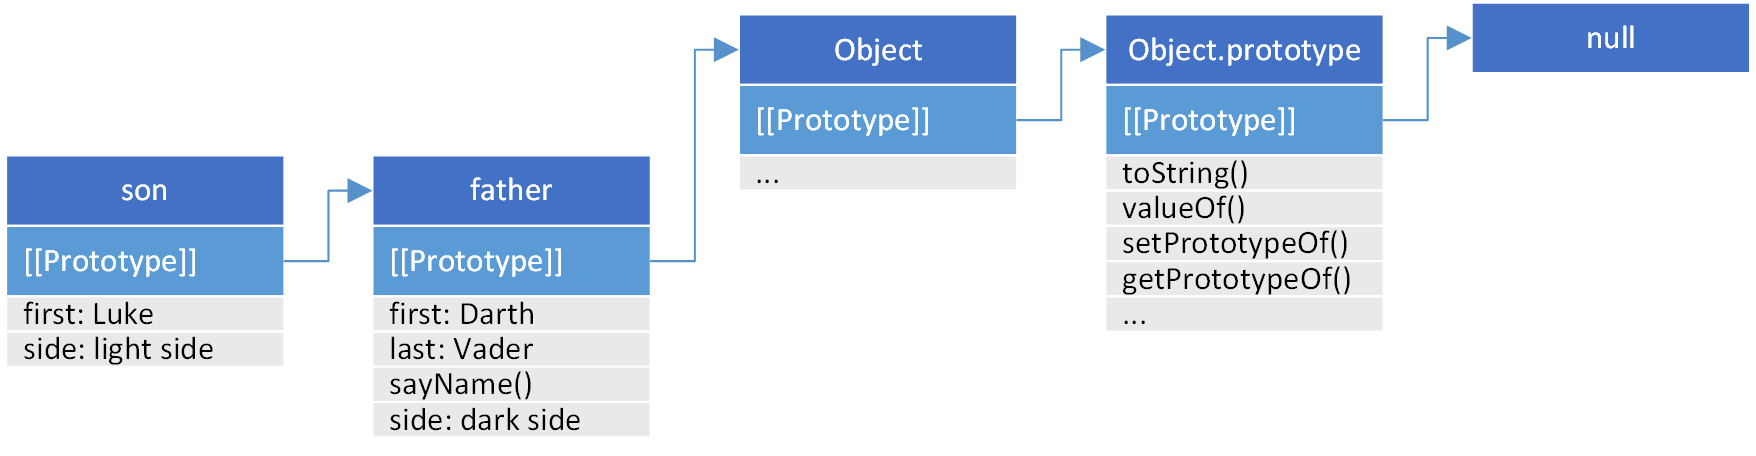
\includegraphics[width=0.8\textwidth]{images/prototypeChain.png}
%	\caption{\label{prototypeChain}Dlegeations-Links entlalang der Prorotype-Chain (aus \citep[p. 118]{StefanovJavaScriptpatternsbuild2010}}
%\end{figure}
%
%
%Wenn in JavaScript auf die Property eines Objekts, sei es ein primitiver Wert oder eine Objektreferenz, zugegriffen wird, so wird zunächst überprüft ob das Objekt eine eigene Property des gewünschten Namens besitzt. Ist dies der Fall, so erfolgt der Zugriff darauf. Ist keine eigene Property des gewünschten Namens vorhanden, so wird im [[Prototype]] des Objekts nachgesehen, ob die gesuchte Property dort vorhanden ist.
%Da auch das [[Prototype]]-Objekt selber ein Objekt ist enthält es auch selber eine Referenz auf ein weiteres [[Prototype]]-Objekt, das in der Hierarchie weiter oben steht. Es entsteht die sogenannte \emph{Prototype-Chain}, entlang derer JavaScript nach einer gewünschten Property sucht, bis diese entweder gefunden wird, oder aber das oberste Objekt der Prototype-Chain als eigenen [[Prototype]] einen Verweis auf \texttt{null} besitzt und die Kette damit am Ende ist. Erst wenn entlang dieser Kette die gewünschte Property nicht gefunden wird, stellt die JavaScript Laufzeitumgebung fest, dass eine Property nicht vorhanden ist und gibt \texttt{undefined} zurück.
%
%Mittels dieses Mechanismus von JavaScript lässt sich auf natürliche Weise eine Delegationshierarchie aufbauen: Gemeinsam genutzte Properties und Methoden werden in einem Objekt definiert, das in den Kind-Objekten, die diese nutzen wollen, als [[Prototype]] referenziert wird. Dadurch können alle Kind-Objekte die auf dem [[Prototype]] definierten Properties und Methoden benutzen. Wenn in einem Objekt für eine Property ein verändertes Verhalten erwünscht ist, so kann einfach eine eigene Property gleichen Namens angelegt werden, welche die ansonsten gemeinsam genutzte Property verdeckt (\emph{shadowing}) und damit deren Verhalten überschreibt.
%
%Änderungen des [[Prototype]] haben Auswirkungen auf alle darauf referenzierenden Objekte, es sei denn die geänderte Property wird weiter unten in der Hierarchie durch eine eigene Property verdeckt. Daher ist bei der Zuweisung von Werten darauf zu achten, ob man gerade auf eine eigene Property zugreift oder auf eine in der Prototype-Chain weiter oben liegende. 
%%Dies kann mittels der Funktion \texttt{Object.prototype.hasOwnProperty()} überprüft werden. 
%
%Wenn es darauf ankommt zu wissen, ob ein Objekt eine Property selber besitzt, oder per Delegation entlang der Prototype-Chain darauf zugreift, so kann dies über die Methode \texttt{obj.hasOwnProperty(prop)} geprüft werden. Diese ist definiert als \texttt{Object.proto\-type.hasOwnProperty()} und wird daher auf einem Objekt \texttt{obj} per Delegation an \texttt{Object.prototype} aufgerufen. Seit der Version ES6  können die eigenen Properties eines Objekts über die funktion \texttt{Object.keys(obj)} als Array abgefragt werden.\footnote{Genau genommen beziehen sich die beiden genannten Funktionen lediglich auf Objektproperties, die als \texttt{enumerable: true} gekennzeichnet sind.}


JavaScript hat einen eingebauten Delegationsmechanismus bezüglich des Zugriffs auf Objekt-Properties. Dazu hat jedes Objekt eine interne Referenz --in der Sprachspezifikation \citep[§9.1]{international2018ecmascript} als \emph{[[Prototype]]}"~Slot bezeichnet-- die entweder auf ein anderes Objekt zeigt oder den primitiven Wert \texttt{null} enthält. Das referenzierte Objekt wird \emph{Prototyp} genannt. Da ein so referenziertes Objekt selber wieder eine Referenz auf einen eigenen Prototypen enthält, ergibt sich eine verkette Liste aus Objekt-Referenzen, die als \emph{Prototype-Chain} bezeichnet wird. 
In der Regel endet die Prototype-Chain im Objekt \texttt{Object.prototype}, auf dem einige nützliche Hilfsfunktionen (z.~B. \texttt{toString() oder \texttt{valueOf()}}) als Properties implementiert sind.

Der Prototyp eines Objekts wird automatisch bei der Objekterzeugung gesetzt und kann über \texttt{Object.getPrototypeOf()} abgefragt bzw. über \texttt{Object.setPrototypeOf()} geändert werden. 
Wie die automatische Setzung erfolgt, wird später im Abschnitt zur Objekterzeugung detailliert erläutert.

Bei einem lesenden Zugriff oder einem Funktionsaufruf auf eine Objekt-Property wird zunächst durch die Runtime geprüft, ob das Objekt selber eine Property entsprechenden Namens hat. Ist dies nicht der Fall, so folgt die Runtime der [[Prototype]]-Referenz und sucht im Prototyp-Objekt nach der passenden Property. Wenn diese dort gefunden wird, so erfolgt der Zugriff darauf. Andernfalls wird die Suche nach der Property entlang der Prototype-Chain fortgesetzt, bis sie entweder gefunden wird, oder die Kette endet. Dieser automatische Zugriff auf Properties von Objekten, die in der Prototypen-Hierarchie weiter oben stehen, entspricht einer Delegation an ein anderes Objekt und umfasst insbesondere auch Methodenaufrufe.

Diese automatische Delegation erfolgt nur bei lesenden Zugriffen auf Properties. Da schreibende Zugriffe auf eine Property Auswirkungen auf alle, in der Prototype-Chain tiefer liegenden Objekte haben, werden Änderungen per Delegation von einem tiefer liegenden Objekt aus verhindert. Bei einem schreibenden Zugriff auf eine Property, die weiter oben in der Prototype-Chain definiert und nicht als \emph{read-only} markiert ist, wird auf dem Startobjekt der Prototype-Chain eine neue Property des gleichen Namens angelegt. Diese neue Property verdeckt bei darauffolgenden lesenden Zugriffen die weiter oben liegende Property des Prototypen. Man spricht in diesem Fall von \emph{shadowing}.\footnote{Der Vollständigkeit halber sei erwähnt, dass eine weiter oben in der Chain liegende Property in Ausnahmefällen verändert werden kann, wenn diese nicht als normale Property, sondern über einen \emph{Setter} definiert ist. Dies ist in der Praxis jedoch die Ausnahme und wird daher hier nicht weiter ausgeführt. Details finden sich in \citep[p. 88f.]{SimpsonThisobjectprototypes2014} und in \citep{international2018ecmascript}.}

Änderungen direkt am Prototypen-Objekt dagegen haben Auswirkungen auf alle darauf referenzierenden Objekte, es sei denn, die geänderte Property wird weiter unten in der Hierarchie verdeckt. Daher ist bei der Zuweisung von Werten darauf zu achten, ob man gerade auf eine eigene Property zugreift oder auf eine in der Prototype-Chain weiter oben liegende. 
Wenn es darauf ankommt zu wissen, ob ein Objekt eine Property selber besitzt, oder per Delegation entlang der Prototype-Chain darauf zugreift, so kann dies über die Methode \texttt{obj.hasOwnProperty(prop)} geprüft werden. Diese ist definiert als \texttt{Object.proto\-type.hasOwnProperty()} und wird daher auf einem Objekt \texttt{obj} per Delegation an \texttt{Object.prototype} aufgerufen. Seit der Version ES6  können die eigenen Properties eines Objekts über die Funktion \texttt{Object.keys(obj)} direkt als Array abgefragt werden (siehe \citep[§19.1.2.16]{international2018ecmascript}).%\footnote{Genau genommen beziehen sich die beiden genannten Funktionen lediglich auf Objektproperties, die als \texttt{enumerable: true} gekennzeichnet sind.}

\skippingparagraph

\insertcode{codesnips/prototypeChain.js}{Beispiel von Delegation und Shadowing in der Prototype Chain}

Zur Verdeutlichung sei hier ein kleines Beispiel angegeben. In Listing \ref{codesnips/prototypeChain.js} wird ein \texttt{father} und ein \texttt{son}-Objekt erstellt. Die [[Prototype]]-Referenz von \texttt{son} wird explizit auf \texttt{father} gesetzt und hat damit per Delegation Zugriff auf dessen Properties inklusive der Methode \texttt{sayName()}. 

Zunächst hat \texttt{son} keine eigenen Properties, kann aber per Delegation auf die Properties von \texttt{father} zugreifen. Die Zuweisung in Zeile 14 erzeugt eine neue Property \texttt{first} auf dem Objekt \texttt{son}, welche die gleichnamige Property von \texttt{father} überdeckt. In Zeile 20 wird \texttt{father.name} geändert. Das hat auch (häufig ungewollte) Auswirkungen auf den Property-Lookup des \texttt{son}-Objekts aus. In den Zeilen 24-31 sind weitere Ausgaben zu sehen, die das Verhalten verdeutlichen. In Abbildung \ref{prototypeChain} ist die Prototype-Chain ausgehend von \texttt{son} zum Programmende schematisch dargestellt.

\begin{figure}[h]
	\centering
	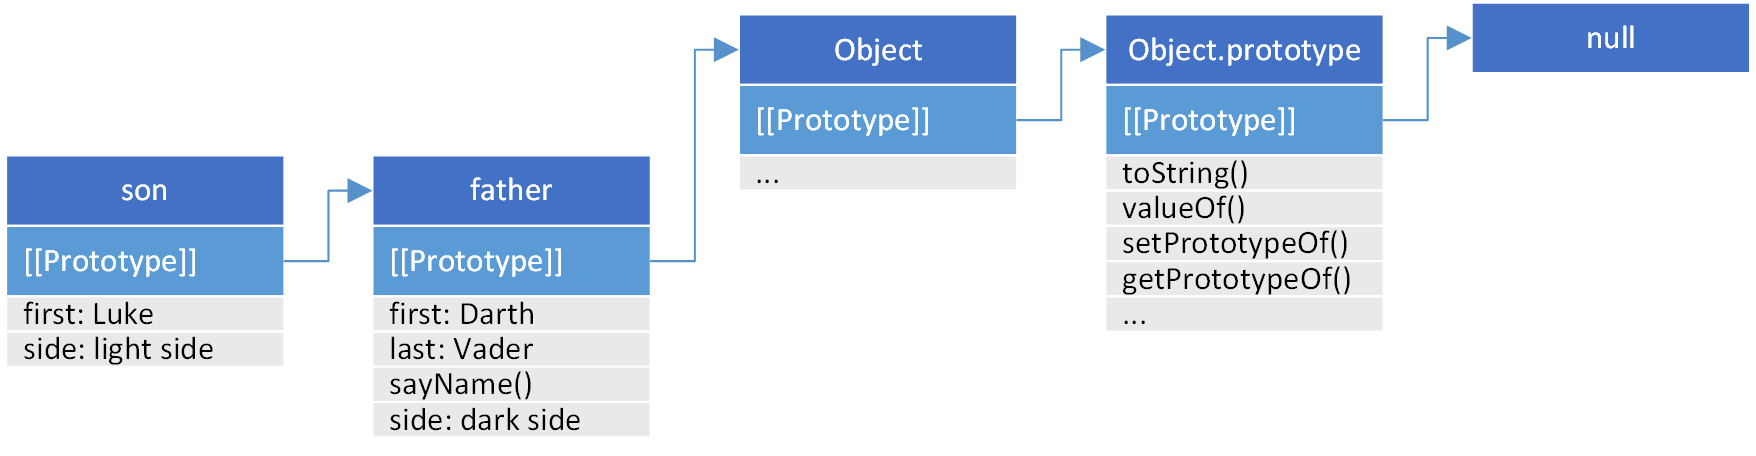
\includegraphics[width=1\textwidth]{images/prototypeChain.png}
	\caption{\label{prototypeChain}Die Prototype-Chain der Objekte aus Listing \ref{codesnips/prototypeChain.js}.}
\end{figure}



%Mittels der beschriebenen Mechanismen von JavaScript lässt sich auf natürliche Weise eine Delegationshierarchie aufbauen: Gemeinsam genutzte Properties und Methoden werden in einem Prototyp-Objekt definiert, und können von darauf verweisenden Kind-Objekten benutzt werden. Wenn in einem Objekt für eine Property ein verändertes Verhalten erwünscht ist, so kann einfach eine eigene Property gleichen Namens angelegt werden, welche die ansonsten gemeinsam genutzte Property verdeckt (\emph{shadowing}) und damit deren Verhalten überschreibt.


\subsection{\texttt{this}-Binding}

%JS:
%In Js ist das \texttt{this}-Binding etwas speziell und daher mit Vorsicht zu genießen:
%- \texttt{this}-Binding ist etwas speziell und kann sich auf verschiedene Dinge beziehen
%	- 4 Varianten aus Kyle

In OO-Sprachen wird eine Möglichkeit benötigt, mit der eine Methode eines Objekts auf die Properties eben dieses Objekts zugreifen kann. In den meisten OO-Pro\-gram\-mier\-spra\-chen gibt es dazu das Schlüsselwort \texttt{this}\footnote{
Der Name des Schlüsselworts variiert in verschiedenen Sprachen.
}, welches an die gerade aktuelle Objektinstanz gebunden ist. 

Auch JavaScript hat das Schlüsselwort \texttt{this} definiert, welches bei einem Funktionsaufruf zur Laufzeit an ein Objekt gebunden wird. An welches Objekt \texttt{this} gebunden wird, ist davon abhängig wie die Funktion aufgerufen wird. Die konkrete Bindung zur Laufzeit gibt den Kontext vor, in dem die Funktion ausgeführt wird und auf dessen Properties sie Zugriff hat. 

Es gibt im Wesentlichen vier Regeln, nach denen die Laufzeitumgebung entscheidet, auf welches Objekt \texttt{this} referenziert. Diese Regeln werden der Reihe nach geprüft und die zuerst zutreffende Regel wird verwendet, um die passende Referenz in \texttt{this} abzulegen:
\begin{enumerate}
	\item \emph{new binding}
	\item \emph{explicit binding}
	\item \emph{implicit binding}
	\item \emph{default binding}
\end{enumerate}

Zusätzlich gibt es seit der Sprachversion ES6 noch einen Bindungsmechanismus, welcher die aufgezählten Regeln außer Kraft setzt:
ES6 \emph{arrow functions} benutzen einen \emph{lexikalischen Kontext} (\emph{lexical scope}) und damit eine feste \texttt{this}-Bindung, die nicht erst zur Laufzeit erstellt wird.

\paragraph{new binding} Wenn eine Funktion als Konstruktorfunktion mit dem Schlüsselwort \texttt{new} aufgerufen wird, so erzeugt sie ein neues Objekt (siehe unten \ref{Objekterzeugung}). Innerhalb der Konstruktorfunktion wird \texttt{this} an dieses neu erzeugte Objekt gebunden.

\paragraph{explicit binding} Die Bindung von \texttt{this} kann für eine Funktion explizit gesetzt werden. Dazu dienen die eingebauten Funktionen \texttt{Function.prototype.call()}, \texttt{Func\-tion.prototype.apply()} und \texttt{Func\-tion.prototype.bind()}. Diese Methoden aus \texttt{Func\-tion.prototype} binden die \texttt{this}-Referenz an das als erstes Argument übergebene Objekt. Dies wird am Besten anhand eines kleinen Beispiels deutlich:

\insertcode{codesnips/thisBinding.js}{Beispiel für die Wirkung von \texttt{call()} und \texttt{bind()}.}

In diesem Code wird die \texttt{this}-Referenz der Funktion \texttt{speak} explizit an verschiedene Objekte gebunden. 

\paragraph{implicit binding} Wenn eine Funktion direkt auf einem umgebenden Objekt aufgerufen wird, so wird dieses Objekt an \texttt{this} gebunden. Diese Bindung geht verloren, wenn die Funktion nicht direkt auf diesem Objekt aufgerufen wird, weil sie z. B. vorher einer anderen Variable zugewiesen wurde (Siehe Beispiel in Listing \ref{codesnips/thisImplicitBinding.js}).

\paragraph{default binding} Wenn keine dieser drei Regeln zutrifft, dann wird als Binding für \texttt{this} entweder \texttt{undefined} im \emph{strict mode} oder das \emph{global object} verwendet.

\insertcode{codesnips/thisImplicitBinding.js}{Beispiel für \emph{implicit binding} und \emph{default binding}.}

\paragraph{lexical binding} In ES6 wurde eine neue kompakte Schreibweise für Funktionsausdrücke eingeführt, die sogenannten \emph{Arrow}-Funktionen. Ihren Namen verdanken sie ihrer Schreibweise mit dem "`fat arrow"'"~Symbol \texttt{=>}. Neben der kompakteren Schreibweise  gibt es einen wichtigen semantischen Unterschied zu konventionellen Funktionen da eine neue Regel für die Bindung von \texttt{this} hinzu kam: Arrow-Funktionen übernehmen für ihr \texttt{this}-Binding das \texttt{this}-Binding des sie umgebenden lexikalischen Kontexts zur Definitionszeit (lexical binding). Dadurch ist es möglich ad-hoc definierte Funktionen, wie sie häufig für Callbacks eingesetzt werden, mit einer sinnhaften Bindung zu versehen, ohne dies explizit zu formulieren. Der Unterschied zu traditionellen Funktionen wird in Listing \ref{codesnips/thisArrowBinding.js} deutlich:

\insertcode{codesnips/thisArrowBinding.js}{Beispiel für das lexical Binding von \texttt{this} in Arrow-Funktionen.}


\subsection{Objekterzeugung}\label{Objekterzeugung}

In den vorangegangenen Abschnitten wurde erläutert, was ein Objekt ist, welche Properties es enthält, wie Delegationshierarchien zwischen Objekten über die Prototype-Chain aufgebaut werden können und wie über das Schlüsselwort \texttt{this} aus einer Methode auf Properties des Objekts zugegriffen werden kann. Bisher wurden jedoch noch kein Überblick darüber gegeben, wie Objekte erzeugt werden können. Dies soll nun nachgeholt werden.

%Klassisch:
%- Ein Objekt wird nurch ein Schlüsselword (meist \texttt{new}) erzeugt und dadurch wird eine Konstruktor aufgerufen
%- Ein einmal definiertes Objekt bleibt, wie es ist.

Auch bei der Objekterzeugung ist es gut, zunächst die weiter verbreiteten klassischen OO-Sprachen zu betrachten, und davon ausgehend die Wege der Objekterzeugung in JavaScript und deren Unterschiede aufzuzeigen.

In klassischen Sprachen ist der Bauplan des Objekts über die Klassendefinition vollständig festgelegt. Zur Laufzeit muss aus diesem Bauplan ein konkretes Objekt instantiiert werden. Dazu wird in den meisten OO-Sprachen eine Konstruktorfunktion zusammen mit dem Schlüsselwort \texttt{new} aufgerufen. Daraufhin wird Speicherplatz für eine neue Instanz des in der Klasse definierten Objekts reserviert und die Konstruktorfunktion wird gestartet. In der Konstruktorfunktion können Initialisierungen der Properties des Objekts vorgenommen werden, bevor am Ende eine Referenz auf das neu instantiierte Objekt zur weiteren Verwendung zurückgegeben wird.

Ein so entstandenes Objekt kann zwar in den konkreten Werten seiner Properties jederzeit verändert werden, die Struktur des Objekts bleibt aber bis zum Ende seiner Lebensdauer unverändert. Ein Objekt ist strukturell immer eine genaue Kopie seiner Klassendefinition und damit in seiner Struktur statisch.

\skippingparagraph

%JS: 
%- Ein Objekt wird erzeugt durch 
%	- "`Out of thin Air"': Durch ein Objektliteral
%	- den Aufruf einer Konstruktorfunktion mit \texttt{new}
%	- Mittels des nachgebildeten Klassenmechanismus durch Definition mit \texttt{class} und anschließendem \texttt{new Class}
%	- \texttt{Object.create\{\}}; Klonen eines Objekts (Setzen des Prototyps)
%- einem Objekt können später beliebige Properties hinzugefügt (oder auch wieder genommen/gelöscht) werden.
%- Objekte sind vollständig dynamisch

In JavaScript dagegen sind Objekte dynamische Gebilde, deren Struktur zur Laufzeit verändert werden kann. Sie können jederzeit angelegt und verändert werden, ohne dass es dazu einer vorher festgelegte Strukturdefinition (in Form einer Klassendefinition) bedarf. Zur Objekterzeugung gibt es verschiedene Methoden, die bezüglich der daraus resultierenden Objekte gleichwertig sind. 

\paragraph{Objektliterale} Die einfachste und am häufigsten eingesetzte Methode zur Objekterzeugung setzt darauf das Objekt einfach aufzuschreiben und ein sogenanntes Objektliteral im Quelltext zu platzieren. Dabei werden die 
Properties des Objekts als \emph{\texttt{\{key: value\}}-Pairs} im Quelltext in geschweiften Klammern angegeben. Daraus wird automatisch ein Objekt erzeugt, welches sich sofort benutzen lässt. Die per Objektliteral erzeugten Objekte werden vom eingebauten Basisobjekt \texttt{Object} abgeleitet; es wird also die [[Prototype]]-Property des neuen Objekts auf \texttt{Object.prototype} gesetzt.

\insertcode{codesnips/objectLiteral.js}{Erzeugung von Objekten mit Objektliteralen. Zunächst wird ein leeres Objekt \texttt{empty} erzeugt. Das Objekt \texttt{foo} dagegen hat mehrere Properties, die entweder primitive Werte oder Objekte sein können.}

\paragraph{Objekterzeugung über Konstruktorfunktionen} In JavaScript kann jede Funktion als Konstruktorfunktion verwendet werden, wenn sie mit dem Schlüsselwort \texttt{new} aufgerufen wird. Zudem hat jede Funktion neben ihrem eigenen impliziten [[Proto\-type]]-Link noch eine explizite \texttt{.prototype}-Property, die auf ein Objekt verweist, das, bei Verwendung der Funktion als Konstruktorfunktion, als Prototyp des neu erzeugten Objekts dient. Auf diesem Prototyp-Objekt können Properties definiert werden, die neu erzeugte Objekte per Delegation erben sollen. Standardmäßig ist das \texttt{.prototype}-Objekt einer neu definierten Funktion ein leeres Objekt \texttt{\{\}}, dessen eigener \texttt{.\_\_proto\_\_}-Link auf \texttt{Object.prototype} referenziert.

Bei einem Aufruf einer Funktion mit \texttt{new} laufen vor der Funktionsausführung einige vorbereitende Schritte ab: Es wird zunächst ein neues, leeres Objekt erzeugt. Dessen impliziter [[Prototype]]-Link wird auf das durch die \texttt{.prototype}-Property der Konstruktorfunktion referenzierte Objekt gesetzt. Das Schlüsselwort \texttt{this} wird an dieses neu erzeugte Objekt gebunden (\emph{new binding}), bevor die aufgerufene Konstruktorfunktion tatsächlich ausgeführt wird. Am Ende der Funktionsausführung wird \texttt{this} implizit zurückgegeben, falls die Funktion nicht per explizitem \texttt{return}-Statement einen anderen Rückgabewert definiert. 
Während der Funktionsausführung kann auf das neue Objekt über die \texttt{this}-Referenz zugegriffen werden und das Objekt kann verändert und seine Properties initialisiert werden.

Eine Konstruktorfunktion unterscheidet sich nicht von einer normalen Funktion. Eine Funktion wird erst durch den Aufruf mit dem Schlüsselwort \texttt{new} zu einer Konstruktorfunktion. Daher ist bei der Verwendung von Konstruktorfunktionen zur Objekterzeugung besondere Vorsicht geboten, diese auch tatsächlich mit dem Schlüsselwort \texttt{new} aufzurufen. Andernfalls wird zwar die Funktion ausgeführt, es wird jedoch vor der Funktionsausführung kein neues Objekt erzeugt und die \texttt{this}-Referenz zeigt per \emph{default binding} auf das globale Objekt (im \emph{non-strict mode}) oder auf \texttt{undefined} (im \emph{strict mode}). In beiden Fällen verhält sich das Programm anders als erwartet, und in komplexeren Anwendungen entstehen dadurch häufig sehr subtile, schwer zu entdeckende Fehler. Per Konvention sollen Konstruktorfunktionen immer mit einem Großbuchstaben beginnen. Es kann per Linter-Regel --also mittels einer rein statischen Codeanalyse\footnote{siehe dazu \url{https://de.wikipedia.org/wiki/Lint_(Programmierwerkzeug)}}-- geprüft werden, dass jeder Aufruf einer Funktion, die mit Großbuchstaben beginnt, auch mit einem \texttt{new} versehen ist (siehe dazu \citep[p. 96]{SimpsonThisobjectprototypes2014}).

\insertcode{codesnips/constructorFunction.js}{Erzeugung eines Objekts über eine Konstruktorfunktion. Da Kon\-struk\-tor\-funk\-tio\-nen gewöhnliche Funktionen sind, führt ein vergessenes \texttt{new} zu unerwarteten Effekten.}

%{\smaller
%Das Schlüsselwort \texttt{new} wird auch verwendet um eine Instanz einer in ES6 eingeführten Klasse zu erzeugen. Darauf soll hier nicht weiter eingegangen werden, da hinter den Kulissen auch nur eine Konstruktorfunktion aufgerufen wird und lediglich der Eindruck von Klassen mit den Mitteln der prototypenbasierten Programmierung nachgebildet wird. 
%}


\paragraph{Erzeugung eines neuen Objekts mit Object.create()} Mit ES6 wurde die neue Funktion \texttt{Object.create()} eingeführt. Sie erzeugt ein neues, leeres Objekt und setzt dessen [[Prototype]]-Property auf das als erstes Argument übergebene Objekt. Damit hat das neu erzeugte Objekt über Delegation entlang der Prototype-Chain alle Eigenschaften des übergebenen Prototypen geerbt und kann dann mit weiteren Properties angereichert werden, oder es können bestimmte (default-)Properties überschrieben werden.\footnote{
In pre-ES6 Laufzeitumgebungen kann der Prototyp eines Objekts auch mittels \texttt{Object.setPrototypeOf()} verändert werden. Dies ist im dritten Beispiel in Listing \ref{codesnips/objectCreate.js} gezeigt. Das ist jedoch vergleichsweise langsam und sollte vermieden werden, da moderne Laufzeitumgebungen viele Optimierungen darauf nicht anwenden können. Siehe dazu  \citep{MozillaDeveloperNetworkObjectsetPrototypeOf}.
}

\insertcode{codesnips/objectCreate.js}{Erzeugung von Objekten per \texttt{Object.create() mit einem spezifischen Prototypen }.}


\paragraph{Factories}

Da in JavaScript jederzeit ein Objekt erzeugt werden kann, ist dies natürlich auch innerhalb von Funktionen möglich. Es ist nicht notwendig eine spezielle Konstruktorfunktion zu schreiben und diese mit \texttt{new} aufzurufen. Es ist völlig ausreichend eine Funktion zu schreiben, die ein neues Objekt erzeugt, mit den passenden Parametern initialisiert und am Ende über ein explizites \texttt{return} Statement zurück gibt. Eine solche Funktion nennt man \emph{Factory}. 

Das gleiche Objekt, das in Listing \ref{codesnips/constructorFunction.js} per \texttt{Dog}-Konstruktor erzeugt wurde, kann auch über eine \texttt{dogFactory} wie in Listing \ref{codesnips/dogFactory.js} erzeugt werden. Bei der Verwendung der \texttt{dogFactory} ist die Programmiererin davor sicher, dass ein vergessenes \texttt{new} Schlüsselwort zu unvorhergesehenen Fehlern führt.

\insertcode{codesnips/dogFactory.js}{Erzeugung eines Objekts über eine Factory. Im Gegensatz zur Erzeugung per Konstruktorfunktionen führt ein vergessenes \texttt{new} \emph{nicht} zu unerwarteten Effekten.}

Die Verwendung von Factories anstelle von Funktionen, die mittels \texttt{new} als Konstruktorfunktionen aufgerufen werden, wird von vielen Autoren massiv präferiert. Begründet wird dies mit einer größeren Sicherheit und Flexibilität gegenüber Konstruktorfunktionen. Die Sicherheit rührt daher, dass \texttt{new} nicht vergessen werden kann, da es niemals benötigt wird. Da der Aufruf einer Factory ohne \texttt{new} und den damit verbundenen Automatismen zur Objekterzeugung erfolgt, ist mit Factories auch eine größere Flexibilität gegeben. Die Art der Objekterzeugung kann besser kontrolliert und gleichzeitig vor der Anwenderin verborgen werden. Damit ist es beispielsweise möglich bei großen und aufwändigen Objekten, deren Erzeugung teuer ist, auf einen Objekt-Pool umzusteigen, in dem nicht mehr benutzte Objekte recycelt werden. Eine solche Änderung ist für die Anwenderin von Factories völlig transparent. Mit Konstruktorfunktionen ist solch eine Änderung von Implementierungsdetails nicht möglich, da neue Objekte vor der Änderung immer mit \texttt{new} erzeugt wurden und nach der Änderung nur noch ohne \texttt{new} abgerufen werden dürfen.

\begin{quote}
Using constructor functions is a clear and strong accent, because
they are completely unnecessary in JavaScript. They are a waste of time and energy.
\citep[p. 51]{ElliottProgrammingJavaScriptapplications2014}
\end{quote}




\skippingparagraph

Auf alle vier angesprochenen Arten lassen sich in JavaScript neue Objekte erzeugen. Bei der Verwendung von Konstruktorfunktionen ist Vorsicht geboten, da ein vergessenes \texttt{new} zu schwer zu lokalisierenden Fehlern führen kann. Objektliterale sind dagegen ein einfaches Mittel, vor allem solche Objekte zu definieren, welche lediglich einmal benötigt werden. Die Erzeugung mittels \texttt{Object.create()} eignet sich bestens, um Objekthierarchien aufzubauen. Diese Methode wird in der Praxis meist innerhalb des \emph{Factory}-Musters eingesetzt. 

Eine wichtige Eigenschaft und ein starkes Differenzierungsmerkmal von JavaScript ist die Tatsache, dass Objekte dynamische Gebilde sind, die sich jederzeit zur Laufzeit verändern lassen. In klassischen Sprachen sind Objekte in ihrer Struktur starr festgelegt und es lassen sich lediglich die darin gespeicherten Daten verändern. In JavaScript dagegen kann zu jeder Zeit jedem Objekt eine weitere Property hinzugefügt oder aus dem Objekt gelöscht werden. Sogar die Prototype-Chain kann zur Laufzeit verändert werden. Damit lässt sich das Verhalten eines Objekts unter Beibehaltung der eigenen Daten zur Laufzeit vollständig austauschen. Wie wir später noch sehen werden ist diese Dynamik der Objekte in JavaScript ein mächtiges Werkzeug zur Wiederverwendung von Code. 

Diese Flexibilität durch Dynamik hat jedoch auch ihren Preis: In JavaScript ist es schwierig bis unmöglich, einem Objekt anzusehen, welche Eigenschaften und welches Verhalten gerade aktuell sind. Während in stark typisierten Sprachen schon zur Compile-Zeit geprüft werden kann, ob auf einem bestimmten Objekt bestimmte Operationen ausgeführt werden können, so kann in JavaScript in der Regel nicht durch eine Typprüfung festgestellt werden, welche Eigenschaften ein Objekt unterstützt. Daher muss in der Praxis auf das sogenannte \emph{Duck-Typing} zurückgegriffen werden: Getreu dem Motto "`if it looks like a duck, and it quacks like a duck, it must be a duck”' (\citep[p. 141]{SimpsonThisobjectprototypes2014}) wird dabei nicht der \texttt{Typ} eines Objekts überprüft, sondern es wird lediglich das Vorhandensein der gerade benötigten Eigenschaft getestet. Es ist ausreichend, wenn diese Eigenschaft benutzt werden kann. Der formale Typ des Objekts ist für deren Verwendung nicht wichtig.



%\subsection{Funktionen als 1st-class-values}
%JS:
%In JS sind Funktionen selber Objekte und damit 1st-Class-Values.
%- Funktionen, die Properties eines Objekts sind, nennt man Methoden
%- Funktionen können sowohl Pramaeter als auch Rückgabewert anderer Funktionen sein
%	- Damit sind HOF möglich
%- Da Funktionen reguläre Objekte sind, können sie selber auch Properties enthalten, die z. B. auf weitere Funktionen referenzieren




% !TeX encoding = UTF-8
% !TeX spellcheck = de_DE
% !TeX root = ./mainDoc.tex

\section{Method Borrowing}

JavaScript macht es der Programmiererin sehr leicht, eine bestimmte Methode eines Objekts in einem anderen Kontext (das bedeutet mit einem anderen \texttt{this}-Binding) auszuführen. Damit kann eine für ein Objekt entwickelte Methode auf ein anderes Objekt angewendet und so wiederverwendet werden. 

Nach den im vorigen Abschnitt erläuterten Regeln ist eine Methode normalerweise mit dem Objekt, auf dem sie aufgerufen wird, über das implizite \texttt{this} verbunden. JavaScript bietet die eingebauten Funktionen \texttt{call()} und \texttt{apply()} an, mit denen sich das \texttt{this}-Binding bei einem Funktionsaufruf explizit überschreiben lässt. \texttt{call()} und \texttt{apply()} unterscheiden sich lediglich darin, wie die Parameter des Funktionsaufrufs übergeben werden. Bei \texttt{call()} werden sie als Parameterliste angegeben während sie bei \texttt{apply()} als Array übergeben werden.
Dies wird an einem Beispiel deutlich:

\insertcode{codesnips/callBorrowing.js}{Die Methode \texttt{doStuff()} des Objekts \texttt{notmyobj} wird aufgerufen und explizit per \texttt{call(myobj)} bzw. \texttt{call(myobj)} an ein anderes Objekt gebunden.
(Beispiel aus \citep{StefanovJavaScriptpatternsbuild2010})}.

Man spricht bei der gezeigten Technik von \emph{method borrowing}, da sich ein Objekt eine Methode eines anderen Objekts ausleiht.

Diese Technik wird sehr häufig angewendet, um Funktionen eingebauter Objekte,  z.~B. des \texttt{Array}-Objekts zu benutzen, obwohl das Objekt, auf dem operiert wird, selber kein Array, sondern nur \emph{array-like} ist. Die innerhalb von Funktionen belegte Variable \texttt{arguments} ist ein solches array-like Objekt (siehe \citep{MozillaDeveloperNetworkargumentsobject}). Um es in ein \emph{echtes} Array umzuwandeln, kann die \texttt{slice()} Methode aus \texttt{Array.prototype} ausgeliehen werden:
\insertcode{codesnips/toArray.js}{Die Methode \texttt{Array.prototype.slice} wird ausgeliehen und auf das array-like \texttt{arguments} Objekt angewendet.}

Wenn eine Funktion in einer Variable gespeichert werden soll oder als Callback übergeben und später aus einem anderen Kontext heraus aufgerufen wird, so verliert sie ihr \texttt{this}-Binding. \texttt{this} fällt beim Aufruf auf das default-Binding zurück, das im non-strict-Mode auf das \emph{global Object} zeigt und im strict-Mode zu einem Laufzeitfehler führt. Um eine Funktion fest an einen Kontext zu binden, gibt es seit ES5 die Funktion \texttt{Function.prototype.bind()}, die es erlaubt ein festes Objekt als \texttt{this}-Binding und optional weitere Funktionsparameter zu fixieren.
\insertcode{codesnips/bindExample.js}{\texttt{bind()} zur festen \texttt{this}-Bindung (Beispiel frei nach \citep{StefanovJavaScriptpatternsbuild2010})}

Die aus dem Objekt \texttt{one} geborgte Methode wird zunächst ungebunden in eine Variable gespeichert (l.~12), so dass ihr \texttt{this} beim Aufruf auf das globale Objekt zeigt, das keine Property \texttt{name} besitzt. Per \texttt{call()} kann das \texttt{this}-binding explizit gesetzt werden (l.~14). Optional kann auch die Funktion vor dem Speichern in einer Variablen fest an ein bestimmtes Objekt gebunden (l.~17) und zusätzlich mit festen Funktionsparametern (l.21) versehen werden. Eine derart fest gebundene Funktion kann auch problemlos als Parameter für Callbacks verwendet werden.



%
%
%Wenn einfach eine funktion wieder verwendet werden soll, so macht es JavaScript der Programmiererin leicht:
%In JS kann jede Funktion mit einem beliebigen Kontext aufgerufen werden. Der Kontext ist dabei das \texttt{this}-Binding. Üblicherweise ist das \texttt{this}-Binding über eine der oben genannten Regeln festgelegt.
%
%Es kann jederzeit ein anderer Kontext per explicit-Binding festgelegt werden. Damit können vorhandene Funktionen eines anderen Objekts ausgeliehen werden.
%
%Sehr üblich ist das bei eingebauten Funktionen, die aber auf dem aktuellen Objekt nicht über die Prototype-Chain ereichbar sind.
%
%Beispiel Array.prototype.slice ist auf \texttt{arguments} nicht verfügbar, da \texttt{arguments}, zwar ein Array-like Object ist, nicht auf die Array-funktionen aus \texttt{Array.prototype} zugreifen kann. (\citep{argumentsobject})
%
%Das geht auch bei eigenen Funktionen und Objekten. Hier ein Beispiel aus \citep{BorrowingMethodsJavaScript}:
%
%
%Anstelle von Borrowing ist es bei eigenen Funktionen besser ein Modul anzulegen und die Funktion von dort zu importieren. \todoCite{\citep[p.86]{ElliottProgrammingJavaScriptapplications2014}}
%



% !TeX encoding = UTF-8
% !TeX spellcheck = de_DE
% !TeX root = ./mainDoc.tex

\section{Delegation und Mixins}

Ein Mechanismus zum Code-Reuse in klassischen Sprachen ist die Vererbung. Dazu wird eine Hierarchie aufeinander aufbauender Klassendefinitionen definiert. Die tiefer liegende Subklassen \emph{erben} alle Eigenschaften der darüber liegender Superklassen und können sie verwenden. Die tiefer liegenden Subklassen können eigene Eigenschaften ergänzen und Eigenschaften der darüber liegenden Superklassen verändern. Man spricht davon, dass Methoden oder Properties überschrieben werden. Man kann sich das vorstellen, wie Baupläne auf transparentem Papier, die übereinandergelegt werden. 

Wenn eine Instanz einer Subklasse erzeugt wird, so entsteht ein neues Objekt nach der Definition, die sich aus der Summe der Klassendefinitionen der Klassenhierarchie ergibt. Das neue Objekt ist eine materialisierte Kopie dieser Summendefinition.

\subsection{Prototypische Vererbung und Delegation}

Da JavaScript nicht auf Klassen basiert, sondern auf Objekten, die zueinander in Beziehung stehen, ist dieser Mechanismus in der Form nicht verfügbar. Javascript bietet anstelle dessen den \emph{Delegation}-Mechanismus entlang der Prototype-Chain.

%, der häufig auch als Vererbung bezeichnet wird und darauf beruht, dass jedes Objekt in Javascript einen Link zu einem weiteren Objekt hat, der als [[Prototype]]-Link bezeichnet wird. 
%Einen solchen [[Prototype]]-Link besitzt jedes Objekt in Javascript. Dieser Link referenziert entweder ein weiteres Objekt, oder aber den primitiven \texttt{null}-Wert. Die Abfolge dieser Links wird als \emph{Prototype-Chain} bezeichnet und geht vom aktuellen Objekt so lange weiter, bis \texttt{null} erreicht wird. In der Regel ist das letzte in der Prototype-Chain referenzierte Objekt das in JavaScript eingebaute Objekt \texttt{Object.prototype}, dessen [[Prototype]] auf \texttt{null} zeigt.
%
%Mit Hilfe dieses Mechanismus kann man in JavaScript Objektgeflechte aufbauen, die sich ähnlich verhalten wie Klassenhierarchien mit Vererbung in klassischen OO-Sprachen. Technisch gesehen handelt es sich aber nicht um Klassenintantiierungen mit geerbten Eigenschaften, sondern um einen Delegationsmechanismus zwischen Objekten. In \citep[p. 116]{SimpsonThisobjectprototypes2014} wird dies als "`OLOO (objects linked to other objects)"'-Stil bezeichnet.
%
%Um zu verstehen, wie die Prototype-Delegation in JavaScript funktioniert muss man zunächst verstehen, wie der Zugriff auf eine Property eines Objekts abläuft.
%Ein Objekt in JavaScript ist wie ein \texttt{\{key: value\}}-Store organisiert, in dem zu jedem Property-Namen (\texttt{key}) der entsprechende primitive Wert oder eine Referenz auf ein weiteres Objekt (\texttt{value}) gespeichert ist.
%Wenn eine Property oder Methode auf einem Objekt aufgerufen wird, so wird zunächst im Objekt selber geschaut, ob es eine passende Property diesen Namens gibt gibt. Ist das der Fall, so wird der zugehörige Wert zurückgegeben. Wird aber keine passende Property gefunden wird, so folgt JS dem [[Prototype]]-Link des Objekts und schaut in dem dadurch referenzierten Objekt nach der gesuchten Property. So wird die gesamte Prototype-Chain abgesucht, bis sie entweder zu Ende ist, oder die gesuchte Property gefunden wurde. Die Suche wird abgebrochen, sobald eine Property passenden Namens gefunden wurde. Dadurch können Properties am Anfang der Prototype-Chain die Properties von Objekten weiter am Ende der Kette überdecken (\emph{shadowing}). Diese verdeckten Properties können dann nur noch über die direkte Angabe des enthaltenden Objekts zugegriffen werden. 
%
%Während der Traversierung der Prototype-Chain bleibt der \texttt{this}-Zeiger immer an das Ursprungsobjekt am Anfang der Kette gebunden. Das bedeutet, dass auch Funktionen, die am ende der Kette stehen trotzdem auf dem Ursprungsobjekt am Anfang der Kette operieren.



%- Auch JS bietet einen Mechanismus, der als Vererbung bezeichnet wird
%- Dieser läuft über die sogenannte Prototype-Chain
%- Es handelt sich eher um Delegation als um Vererbung
%	- Wenn eine Property oder Methode auf einem Objekt aufgerufen wird, so wird zunächst im Objekt selber geschaut, ob es eine passende Property gibt
%	- Wenn keine passende Property gefunden wird, dann folgt JS dem [[Prototype]] Link und schaut in dem dadurch referenzierten Objekt nach der gesuchten Property
%	- Es wird die gesamte \emph{Prototype-Chain} abgesucht, bis diese entweder zu Ende ist, oder eine passende Property gefunden wurde.
%	- Es wird abgebrochen, sobald eine passende Property gefunden wird.
%	- Wenn es sich um eine Funktion handelt, so ist \texttt{this} immer noch an das Ursprungsobjekt am Anfang der Prototype-Chain gebunden

%\subsection{Prototypische Vererbung über Delegation}

Der [[Prototype]]-Link eines jeden Objekts ist zugreifbar und kann sowohl gelesen als auch gesetzt werden. Der Prototyp ist über die Funktionen \texttt{Object.get\-Proto\-typeOf(obj)} und \texttt{Object.setProto\-typeOf(obj, proto)}, und seit ES6 auch über die eigenen Property \texttt{.\_\_proto\_\_} zugreifbar. Bei Objekten, die über einen Konstruktoraufruf erzeugt werden, wird der [[Prototype]]-Link bei der Erzeugung auf das über die Property \texttt{.prototype} der Konstruktorfunktion referenzierte Objekt gesetzt.

Mit Hilfe der Prototype-Chain und der Möglichkeit, den Prototypen eines Objekts zu manipulieren, lässt sich klassenähnliches Verhalten in JavaScript simulieren: (Wert"~) Pro\-per\-ties werden in der Konstruktorfunktion auf dem neu erstellten Objekt definiert. Sie sind für jedes später über den Konstruktor erzeugte  Objekt genau einmal vorhanden. Methoden (Verhaltens-Properties) werden auf dem Prototypen des Objekts definiert, auf den \texttt{.prototype} der Konstruktorfunktion zeigt. Sie sind lediglich einmal auf dem [[Prototype]]-Objekt vorhanden, auf das alle über den Konstruktor erzeugten Objekte verlinkt sind. Auch auf dem Prototypen können Wert-Properties definiert werden, das funktioniert aber häufig nicht so, wie gewünscht.

Ein Beispiel eines Zählerobjekts ist in Listing \ref{codesnips/protoCounterConstructor.js} zu sehen:

\insertcode{codesnips/protoCounterConstructor.js}{Erzeugung eine \texttt{Counter}-"`Klasse"' und Instantiierung zweier \texttt{Counter}-Objekte.}

Zunächst wird eine Konstruktorfunktion definiert, auf deren \texttt{.prototype}-Objekt die für einen Zähler notwendigen Properties und Funktionen definiert sind.
Sodann werden über Konstruktoraufrufe zwei Zählerobjekte erzeugt. Die Zähler werden mehrfach inkrementiert und das Ergebnis abgefragt. Es ergibt sich folgende (überaschende) Ausgabe:
\begin{verbatim}
one.counter? false
one.counter? true
two.counter = 0;	two.counterObj.value = 3;
one.counter = 3;	one.counterObj.value = 4;
two.counter = 1;	two.counterObj.value = 4;
\end{verbatim}

Diese Ausgabe lässt sich wie folgt erklären: Die Wert-Properties \texttt{counter} und \texttt{coun\-ter\-Obj} sind auf dem Prototypen \texttt{Counter.prototype} definiert. Das durch den Konstruktoraufruf \texttt{new Counter('one');} erzeugte Objekt hat keine eigene Property mit dem Namen \texttt{counter}. Sobald jedoch die Funktion \texttt{inc()} aufgerufen wird, wird eine solche Property direkt auf dem Objekt \texttt{one}, auf das die \texttt{this}-Referenz beim Funktionsaufruf zeigt, angelegt und mit einem Wert belegt. Das liegt daran, das bei schreibenden Zugriffen auf eine Property nicht erst ein passendes Objekt entlang der Prototype-Chain gesucht wird, sondern direkt eine eigene Property angelegt wird, wenn der Schreibzugriff auf eine noch nicht existierende Property des Objekts erfolgt. 

Die Zeile \texttt{this.counter++;} wird ausgeführt als \texttt{one.counter = one.counter + 1}. Es wird die Property \texttt{counter} auf dem Objekt \texttt{one} gesucht und auf \texttt{one.\_\_proto\_\_} gefunden. Dazu wird 1 addiert und es wird der Property \texttt{one.counter} zugewiesen. Da diese Property auf \texttt{one} noch nicht existiert, wird sie angelegt. Ab nun hat \texttt{one} eine eigene Property \texttt{counter}, welche \texttt{one.\_\_proto\_\_.counter} verdeckt.

Die Zeile \texttt{this.counterObj.value} dagegen wird als \texttt{one.counterObj.value = one.} \texttt{counterObj.value + 1} ausgeführt. Hier wird bei beiden Zugriffen auf \texttt{one.counterObj} nur lesend zugegriffen. Der Schreibzugriff erfolgt auf die darin enthaltene \texttt{value}  Property.
In beiden Fällen wird für \texttt{one.counterObj} die Objektreferenz auf \texttt{one.\_\_proto\_\_} gefunden. Die in diesem referenzierten Objekt enthaltene Property \texttt{value} wird ausgelesen, inkrementiert und gespeichert. Die Objektreferenz \texttt{one.counterObj} bleibt dabei unverändert. Sie ist für beide Objekte \texttt{one} und \texttt{two} lediglich einmal auf dem durch \texttt{Counter.prototype} referenzierten Objekt vorhanden.
Die Abbildung \ref{shadowing} veranschaulicht die Situation.
\begin{figure}[!h]
	\centering
	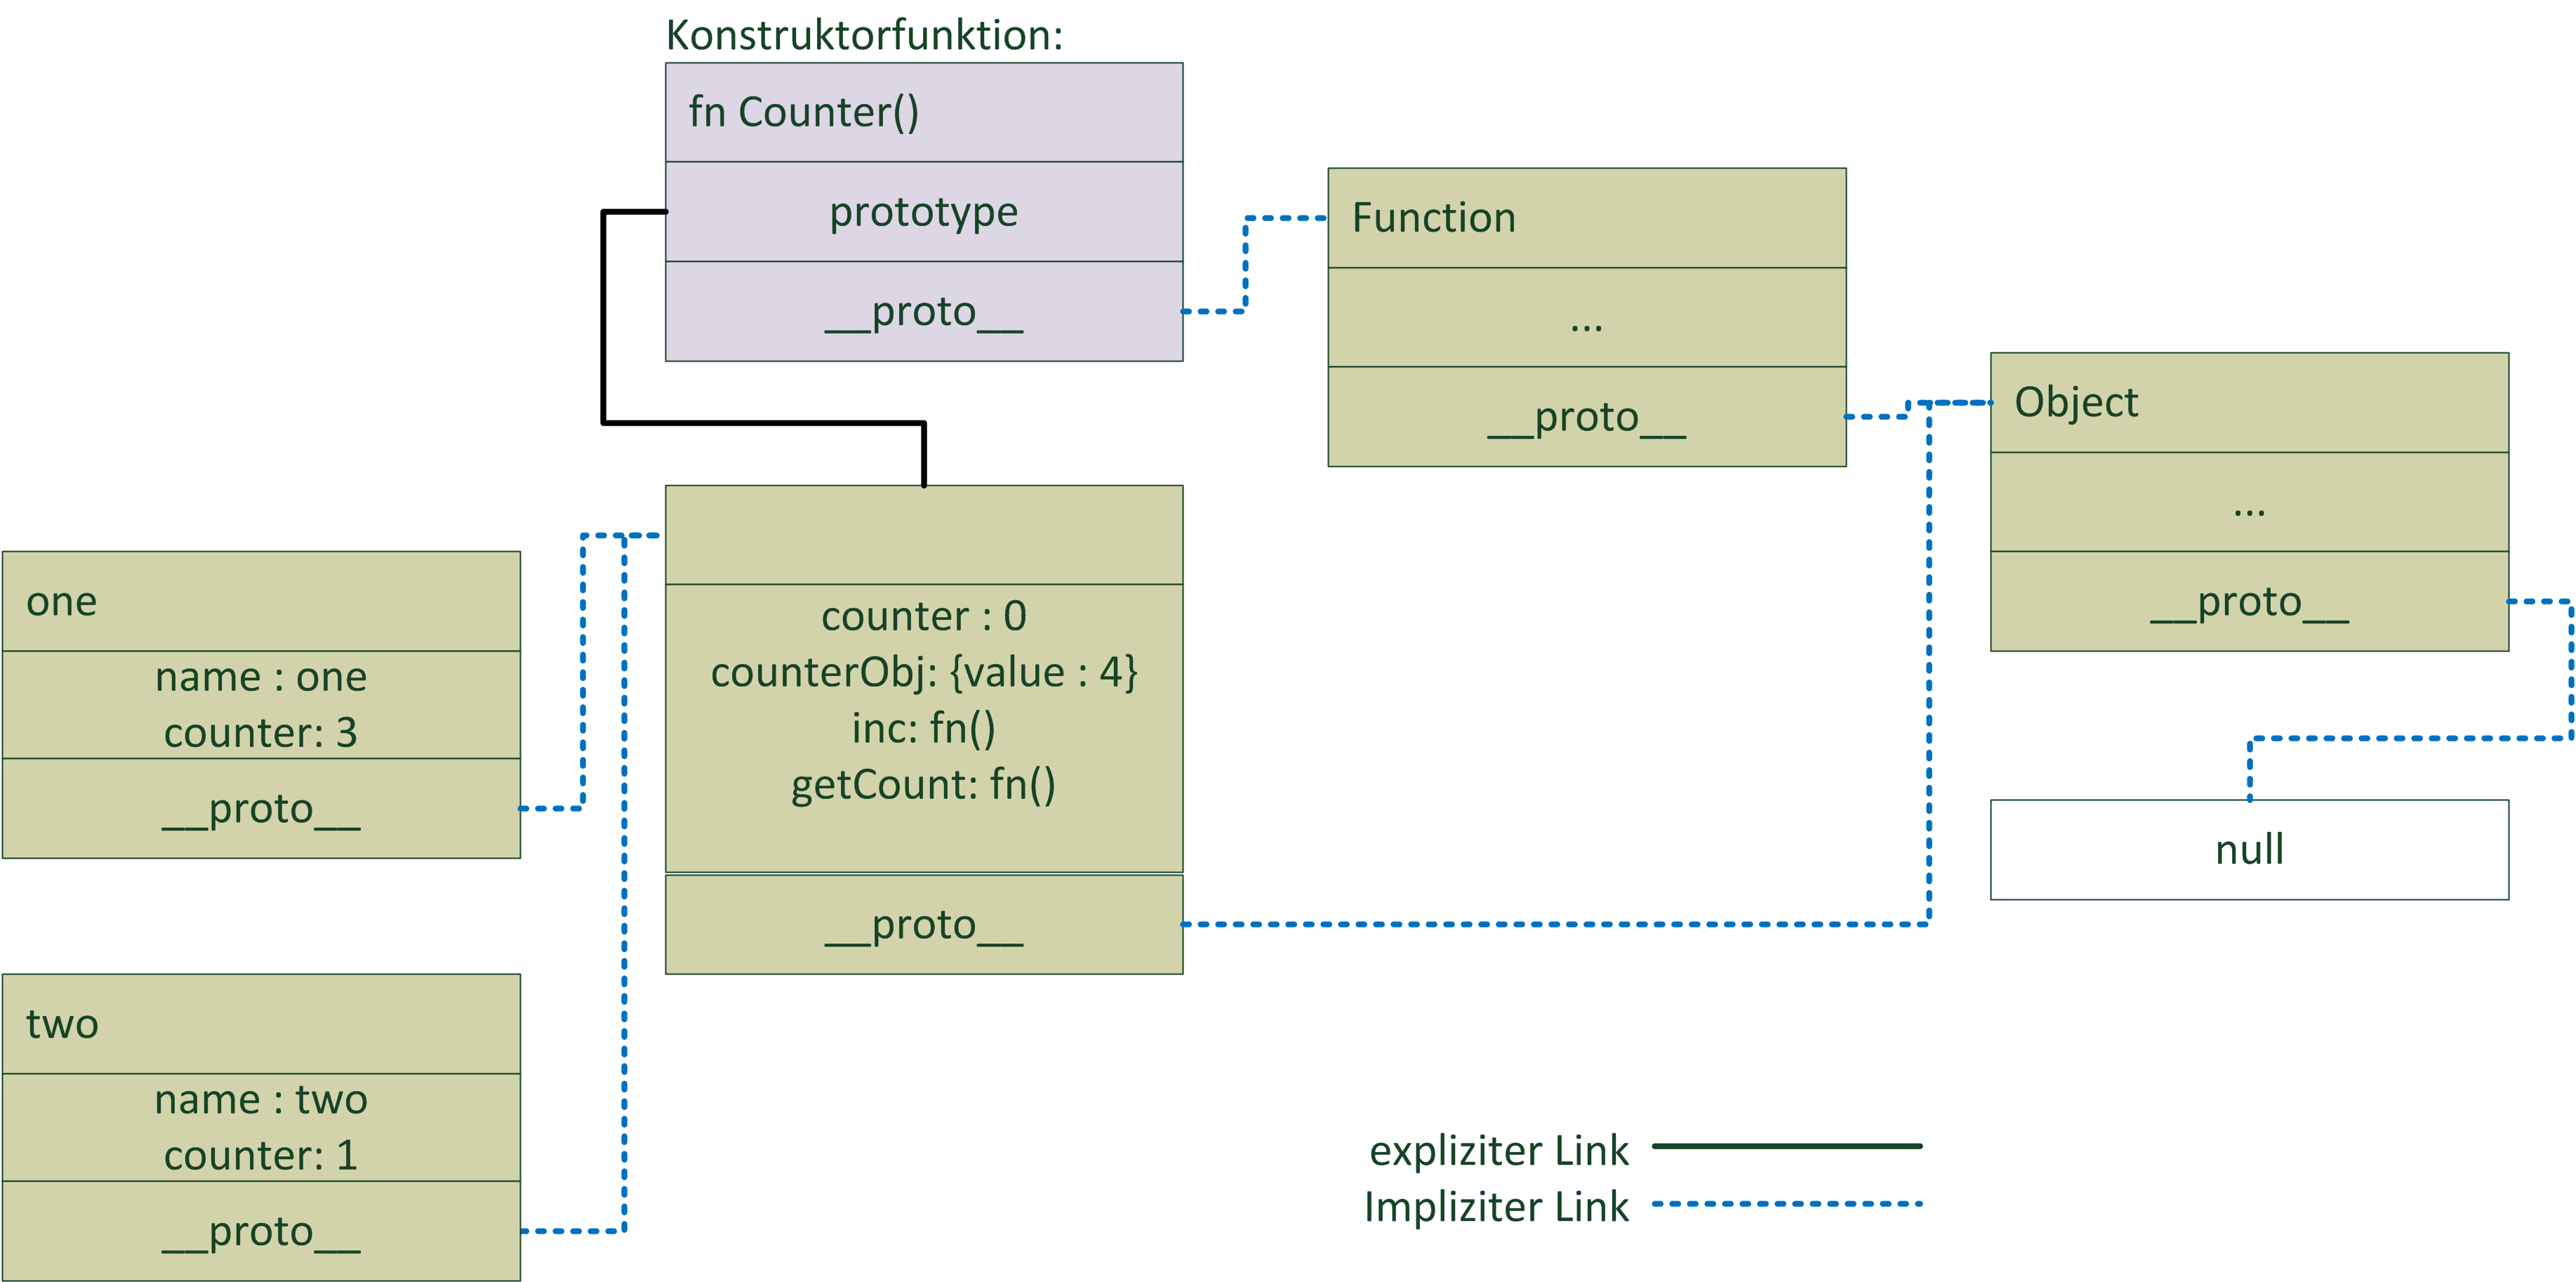
\includegraphics[width=\textwidth]{images/CounterPrototypeChain.png}
	\caption{\label{shadowing}Objektgeflecht des Zählerbeispiels.}
\end{figure}

%In diesem Beispiel wird deutlich, dass die beiden Objekte \texttt{one} und \texttt{two} \emph{nicht} wie in der klassischen Objektorientierung eine materialisierte Kopie der Klassendefinition von \texttt{Counter} sind, die alle Eigenschaften und Properties von \texttt{Counter.prototype} erben, sondern in JavaScript lediglich Objekte exisitieren, die mit anderen Objekten verlinkt sind und über diese Links Aufgaben delegieren. Beim Aufbau von vererbungsähnlichen Delegationshierarchien muss die Programmiererin immer im Auge behalten, auf welchem Objekt eine Property gerade definiert ist und ob es sich um einen primitiven Wert oder eine Referenz handelt.\footnote{Mit der Einführung des Klassenmechanismus über \texttt{class} sind viele Automatismen eingeführt wurden, welche der Programmiererin den Eindruck einer klassischen OO-Sprache vermitteln. Doch auch ES6-Klassen werden unter der Haube auf den dargestellten Delegationsmechanismus abgebildet.}

\skippingparagraph

Ausgehend von dem gezeigt Beispiel lassen sich natürlich auch in JavaScript mehrstufige Delegations-Hierarchien erstellen, die einer Vererbungshierarchie in klassischen OO-Sprachen ähnelt. Zur Verdeutlichung des Prinzips sei ein kurzes Beispiel gezeigt. Es sollen, wie in Abbildung \ref{protoInheritance} dargestellt, vier Objekte erstellt werden.

\begin{figure}[!h]
	\centering
	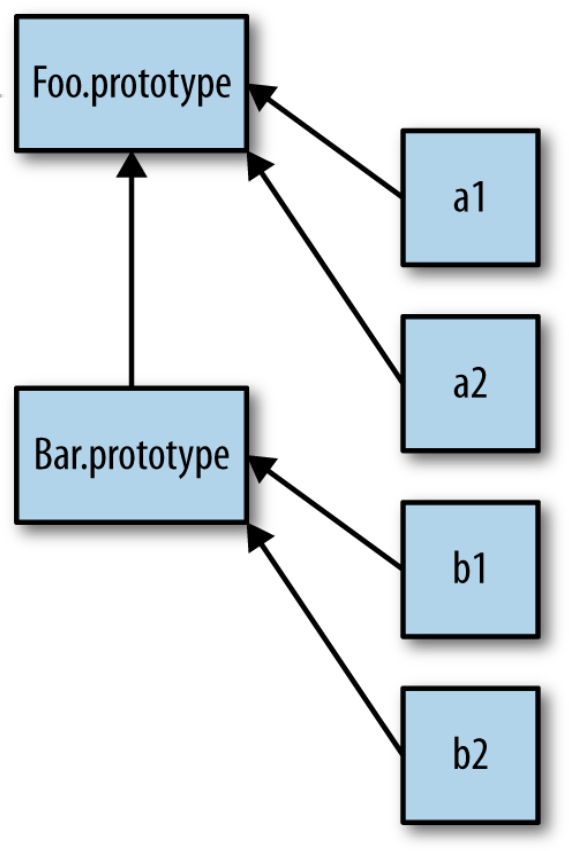
\includegraphics[width=0.3\textwidth]{images/prototypalInheritance.png}
	\caption{\label{protoInheritance}Prototypische Vererbung / Delegationshierarchie (aus \citep[p. 93]{SimpsonThisobjectprototypes2014})}
\end{figure}

Dies lässt sich wie im Listing \ref{codesnips/protoInheritanceSimpson.js} gezeigt programmieren. Zunächst wird eine Konstruktorfunktion für \texttt{Foo} erstellt, auf deren \texttt{.prototpye}-Objekt eine Funktion \texttt{identify} definiert wird. Dieser Prototyp wird als zu verlinkendes Delegate-Objekt an die zweite Konstruktorfunktion \texttt{Bar} über deren \texttt{.prototype}-Link angebunden. Im \texttt{Bar}-Konstruk\-tor wird explizit \texttt{Foo.call(this)} aufgerufen. Es handelt sich dabei um Method-Borrow\-ing, so dass \texttt{Foo} ein explizites \texttt{this}-Binding auf das Objekt erhält, das beim Konstruktoraufruf von \texttt{Bar} neu erzeugt wurde und auf diesem Objekt Properties setzen kann. 

Auch auf dem \texttt{Bar.prototype}-Objekt ist eine Funktion \texttt{identify} definiert. Diese "`überschreibt"' die gleichnamige Funktion auf \texttt{Foo.prototype}, da sie in der Prototype-Chain früher gefunden wird. Es ist zu erkennen, dass der in klassichen Sprachen übliche Aufruf der überschriebenen Funktion deutlich umständlicher ist als der klassisch übliche Aufruf \texttt{super()}. In JavaScript ist man daher bemüht das Überschreiben zu vermeiden, wenn die überschriebene Property noch benötigt wird.


\insertcode{codesnips/protoInheritanceSimpson.js}{Erzeugung einer mehrstufigen prototypischen Vererbungs-/Delegations-Hierarchie (frei nach \citep{SimpsonThisobjectprototypes2014}, p. 101)}


\subsection{Vererbung durch Kopieren}

Im vorangehenden Abschnitt wurde gezeigt, wie die in JavaScript enthaltene Delegation zwischen OLOO (Objects Linked to Other Objects) funktioniert, und wie man mit ihrer Hilfe einen Mechanismus aufsetzen kann, der der klassischen Vererbung sehr nahe kommt. Es wurde dabei im \texttt{Counter}-Beispiel auch aufgezeigt, dass bei der Objektinstantiierung keine Kopien von Klassendefinitionen erstellt werden, sondern lediglich Objekte, die über Ihre Prototype-Chain auf andere, bereits bestehende Objekte verlinkt sind. Dies kann zu unerwartetem Verhalten führen, wenn nicht genau darauf geachtet wird, ob eine Property einen primitiven Wert enthält oder auf ein Objekt refrenziert.

In den vorangehenden Beispielen wurde auch deutlich, dass --im Gegensatz zu klassischen Sprachen-- Objekte in JavaScript dynamisch sind und jederzeit auch nach Erstellung verändert werden können. So wurden den \texttt{.prototype}-Objekten nach ihrer Erstellung Funktions-Properties hinzugefügt.

Die Möglichkeit, Objekte nach ihrer Erstellung zu verändern, lässt sich nutzen, um Code-Wiederverwendung nicht über Delegation zu erreichen, sondern über automatisierte Kopien von Properties. Es lässt sich einfach eine Hilfsfunktion \texttt{extend} schreiben, die ein bestehendes Objekt mit den Properties eines anderen Objekts erweitert. Die Vererbung findet hier durch Kopieren statt.

In Listing \ref{codesnips/extendStefanov.js} wird ein \texttt{kid} Objekt dadurch erzeugt, dass in ein leeres Objekt alle eigenen Properties des \texttt{dad}-Objekts einkopiert werden. Wichtig zu sehen ist dabei, dass diese beiden Objekte \texttt{nicht} über die Prototype-Chain verbunden sind. Es werden lediglich die im Elternobjekt vorhandenen eigenen Properties kopiert. Es wird eine sogenannte \emph{flache} Kopie (\emph{shallow copy}) des Elternobjekts im Kind-Objekt erzeugt. Die gezeigte Funktion \texttt{extend} ist seit ES6 auch im JavaScript Sprachstandard enthalten und es kann einfacher \texttt{Object.assign(target, \ldots sources)} geschrieben werden.

\insertcode{codesnips/extendStefanov.js}{"`Vererbung"' durch Kopieren (frei nach \citep{StefanovJavaScriptpatternsbuild2010}, p. 133f.)}

Auch hier besteht das Problem wie im \texttt{Counter}-Beispiel, dass Properties, die Referenzen auf andere Objekte sind, von beiden Kopien aus auf das gleiche Ursprungsobjekt zeigen und damit keine eigenständigen, gedoppelten Werte enthalten. 
Das ist in der Regel nicht gewünscht, und es müssen entsprechende Setter-Funktionen programmiert werden, die den Inhalt solcher Referenzen durch eigene Objekte ersetzen, und nicht nur den Wert einzelner Objektproperties verändern. In diesem Beispiel sollte die Funktion \texttt{Array.concat()} anstelle von \texttt{Array.push()} verwendet werden. \texttt{Array.concat()} gibt immer ein neues Array zurück, während \texttt{Array.push()} das ursprüngliche Array verändert.

Eine (selten genutzte) Alternative besteht darin, eine sogenannte \emph{tiefe} Kopie (\emph{deep copy}) zu erstellen, die Objekt- und Array-Referenzen rekursiv auflöst, und entsprechend neue Werte im Empfängerobjekt erstellt. Eine solche tiefe Kopierfunktion ist in Listing \ref{codesnips/extendDeepStefanov.js} zu sehen.

\insertcode{codesnips/extendDeepStefanov.js}{"`Vererbung"' durch \emph{tiefes }Kopieren (frei nach \citep{StefanovJavaScriptpatternsbuild2010}, p. 134)}

Mit Hilfe der \texttt{extendDeep} Funktion wird das \texttt{parent}-Objekt im \texttt{child}-Objekt vollständig dupliziert. Dadurch können sich die beiden Objekte danach nicht mehr beeinflussen. Eine solche tiefe Kopie ist jedoch eine sehr teure Operation und meist nicht notwendig. Der Einsatz einer tiefen Kopierfunktion für die Wiederverwendung von Code ist nur in Ausnahemefällen sinnvoll, die im Vorfeld genau analysiert werden müssen. In den meisten Fällen ist die sorgfältige Implementierung geeigneter Setter vorzuziehen, die selektiv Objekte austauschen, wenn darin enthaltene Werte verändert werden sollen.

\subsection{Object-Mixins für den orthogonalen Code-Reuse}
Durch bisher gezeigten Beispiele der Code-Wiederverwendung per Delegation oder per Kopie wurde eine baumartige Hierarchie aufgebaut, wie sie typischerweise in allen Vererbungshierarchien in OO-Sprachen mit Einfachvererbung entsteht. Eine solch strenge Hierarchie, in der jede Entität genau einen Vorgänger hat, von dem Eigenschaften übernommen werden können, ist in der Praxis häufig nicht ausreichend. Es gibt in der Realität in fast allen Bereichen Anwendungsfälle, die sich mit einer solchen Baumstruktur nicht darstellen lassen. %Es gibt Querverbindungen zwischen Modellaspekten, die \emph{orthogonal} zu dieser Baumstruktur stehen.

Als Beispiel sei das Modell einer Firma und ihrer Mitarbeitern genannt: Ein \texttt{Entwick\-ler} ist ein \texttt{Angestellter}, der eine \texttt{Person} ist. Daneben gibt es noch einen \texttt{Produktions\-mitarbeiter}, der ein \texttt{Angestellter} ist, der eine \texttt{Person} ist. Dieses auf den ersten Blick einleuchtende Modell bricht, sobald ein externer \texttt{Entwickler} in der Firma beschäftigt wird, der selber ein \texttt{Freelancer} ist. In diesem Fall  kann die Realität nicht über einen einfachen Baum modelliert werden. Es kommen Eigenschaften hinzu, die zu der ursprünglich verwendeten Taxonomie \emph{orthogonal} sind. 
%In klassischen Sprachen lässt sich solch ein Problem teilweise durch Mehrfachvererbung modellieren. 

Ein Ansatz zur Modellierung solcher orthogonaler Beziehungen, die nicht einer strengen Hierarchie gehorchen, wird als \emph{Mixin} bezeichnet. 

Der Begriff des Mix-In wurde laut Wikipedia\footnote{\url{https://en.wikipedia.org/wiki/Mix-in}} ursprünglich von einem Eis-Verkäufer geprägt, der aus den immer gleichen Grundsorten (Vanille, Schokolade, \ldots) und weiteren Zutaten (Smarties, Schoko-Chips, Gummibärchen, Kekse, \ldots) eine Unmenge an spezialisierten Eiscremesorten anbieten konnte, die individuell nach Kundenwunsch zubereitet wurden. Er benutzte eine Grundsorte als Ausgangsbasis und mixte weitere Zutaten nach Kundenwunsch unter, so dass ein neuer individueller Geschmack entstand. 

Übertragen auf klassische OO-Programmierung, stellen die baumartigen Vererbungshierarchien aus Super- und Subklassen die Grundzutaten dar. Die zusätzlichen Bestandteile werden mit dem dazu orthogonalem Verhalten identifiziert, das je nach Bedarf hinzugefügt werden kann. Das zuzufügende Verhalten kann in der Sprache der klassischen Objektorientierung als Definition einer \emph{abstrakten Subklasse} bezeichnet werden.

\begin{quote}
A mixin is an abstract subclass; i.e. a subclass definition that may be applied to different
superclasses to create a related family of modified classes.  \citep{BrachaMixinbasedInheritance1990}
\end{quote}

Diese abstrakte Subklasse kann für sich gesehen nicht instantiert werden. Sie kann nur auf eine konkrete Basisklasse angewendet werden, und damit ihr Verhalten dem Verhalten der Basisklasse hinzufügen. Die Basisklasse muss dazu bestimmte Garantien bezüglich ihrer Implementierung geben, damit die erweiterte Funktionalität zur Verfügung gestellt werden kann. Die Verwendung von Mixins in klassischen OO-Sprachen bedarf der Unterstützung der Sprache selber, deren Klassendefinitionen und Objektinstantiierung die Idee einer abstrakten Subklasse, die auf eine konkrete Superklasse angewendet wird, implementieren müssen. Die meisten klassischen OO-Sprachen haben ein Modell implementiert, bei der die Konkretisierung von abstrakten Superklassen zu konkreten Subklassen, also von oben nach unten, geht. Dieses Modell lässt sich nicht ohne weiteres umkehren, weswegen Mixins nicht in vielen Sprachen unterstützt werden.\footnote{Eine Liste von Sprachen, die Mixins direkt unterstützen, findet sich z. B. in \url{https://en.wikipedia.org/wiki/Mixin\%23Programming_languages_that_use_mixins}
}


\begin{figure}[h]
	\centering
	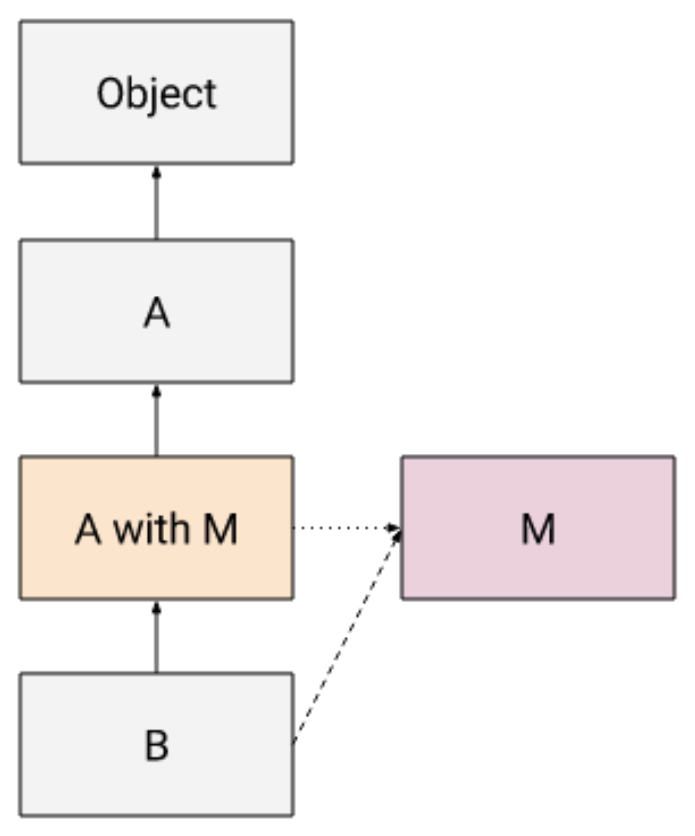
\includegraphics[width=0.3\textwidth]{images/mixinAbstractSubClass.png}
	\caption{\label{mixinAbstractSubClass}Die abstrakte Mixinklasse \texttt{M} angewandt auf die Basisklasse \texttt{A} in der Vererbungshierarchie \texttt{class B extends A with M \{\}}(\citep{FagnaniRealMixinsJavaScript2015})}
\end{figure}

\skippingparagraph

JavaScript hat keine Klassen. Es gibt lediglich Objekte und diese Objekte sind zur Laufzeit dynamisch veränderbar. Damit ergibt sich als direkte Konsequenz aus der im vorigen Abschnitt aufgezeigten einfachen "`Wiederverwendung durch Kopieren"' die Möglichkeit, das Verhalten eines Objekts in ein anderes bestehendes Objekt zu mixen. Der in klassischen Sprachen recht aufwändige Mixin-Mechanismus lässt sich in JavaScript auf eine einfache Kopie zurückführen.

In einer Grundform ist eine flache Kopie der Properties des Mixin-Objekts auf das Empfängerobjekt ausreichend, um eine Mixin-Funktionalität in Javascript zur Verfügung zu stellen. Dieser Vorgang wird auch als "`concatenative sharing"' (\citep{BraithwaiteWhyAreMixins2016}) bezeichnet, da schlicht die Properties des Mixin-Objekts an das zu erweiternde Objekt angehängt werden. In der Vergangenheit wurden dazu meist mehr oder weniger aufwändige \texttt{mixin()}-Funktionen aus Bibliotheken verwendet. Seit ES6 ist jedoch die Funktion \texttt{Object.assign(target, \ldots sources)} standardisiert und kann für diesen Zweck genutzt werden.

Im Listing \ref{codesnips/simpleMixin.js} wird gezeigt, wie leicht sich bestehende Objekte durch einfache Erweiterung mit Mixin-Verhalten ergänzen lassen. Es wird auch deutlich, dass die Mixin-Objekte nicht für sich allein stehen können, da sie im Beispiel auf die \texttt{.name}-Property des Empfängerobjekts zugreifen.

\insertcode{codesnips/simpleMixin.js}{Einfache Object-Mixins durch Definition von Mixin-Objekten und Anwenden von \texttt{Object.assign(target, \ldots sources)}}

Bei der vorgestellten Mixin-Technik werden die Empfängerobjekte lediglich durch eine flache Kopie der Mixin-Objekte erweitert. Es ist daher genau wie im vorangehenden Beispiel darauf zu achten, dass Referenzen auf Objekte innerhalb verschiedener Empfängerobjekte zunächst auf das gleiche Objekt zeigen. Während dieses Verhalten bei den Referenzen auf Funktionen (und damit auf Verhalten des Mixins) wünschenswert ist, um Speicher zu sparen, ist bei objektwertigen Properties Vorsicht geboten. Nach der Erweiterung der beiden Objekte \texttt{felix} und \texttt{john} mit dem \texttt{mixDeveloper} gilt \texttt{john.languages === felix.languages}. 
Das bedeutet, dass die \texttt{.languages}-Property beider Objekte auf dasselbe Array-Objekt referenziert (l.~72). 

Im gezeigten Code-Beispiel wurde dafür Sorge getragen, dass dieses Verhalten keine unerwünschten Nebeneffekte hat. Die \texttt{languages} und \texttt{patterns} Arrays werden bei Veränderung ersetzt und nicht modifiziert. Sowohl die Funktion \texttt{initDeveloper} als auch die Funktionen \texttt{addLanguage} bzw. \texttt{addPattern} ersetzen die Arrays und modifizieren damit die Referenzen der Objekte und nicht nur die Werte innerhalb referenzierter Objekte. 

Aufgrund der Verwendung dynamischer Objekte, deren Verhalten und Struktur zur Laufzeit modifiziert werden kann, ist das Mixin-Pattern in JavaScript sehr einfach anzuwenden. Es bedarf keiner zusätzlichen Sprachunterstützung, sondern lässt sich mit den vorhandenen Mitteln einfach erledigen. Das Muster lässt sich auch in Kombination mit der [[Prototype]]-Delegation einsetzen, so dass nicht nur einzelne Objekte wie im Beispiel mit erweiterter Funktionalität ausgestattet werden können, sondern auch deren [[Prototype]]-Delegates. Dies lässt sich in Factory-Funktionen gewinnbringend einsetzen, wenn eine große Menge erweiterter Objekte erzeugt werden soll. 

\skippingparagraph
Trotz des einfachen Einsatzes von Mixins soll nicht verschwiegen werden, dass in der Praxis in größeren Projekten noch einige Details behandelt werden müssen, die den Einsatz etwas komplizierter als im Beispiel gezeigt machen. Dies betrifft insbesondere den Umgang mit namensgleichen Properties. In der gezeigten Methodik "`gewinnt"' das zuletzt eingemixte Objekt und dessen Implementierung einer Property oder eines Verhaltens bestimmt das Verhalten des erweiterten Objekts. Ohne spezielle Vorkehrungen gibt es keine Möglichkeit, die Methoden oder Properties der Vorgängerobjekte zu erreichen. Es kann jedoch per Method-Borrowing explizit aus der überschreibenden Mixin-Methode die gleichnamige Methode des Empfängerobjekts aufgerufen werden (siehe dazu "`explicit pseudopolymorphism"' \citep[p.78]{SimpsonThisobjectprototypes2014}). Eine andere Möglichkeit besteht darin eine aufwändigere \texttt{mixin()}-Funktion zu benutzen, die bei Namensgleichheit eine automatische Konfliktlösung bietet. Dies wird z.~B. in \texttt{react-server.js} realisiert. Dort können für bestimmte Properties sogenannte \texttt{specPolicies} wie \texttt{OVERRIDE\_BASE}, \texttt{DEFINE\_ONCE}, \texttt{DEFINE\_MANY} oder \texttt{DEFINE\_MANY\_MERGED} angegeben werden. Diese zusätzlichen Angaben werden beim Kopieren der Properties entsprechend berücksichtigt. Die Details dieser Implementierung\footnote{
Die Funktion \texttt{mixSpecIntoComponent} lohnt eine weitere Betrachtung der Mechanismen: \url{https://github.com/reactjs/react-rails/blob/ec9e1736d4aac87afe4c4e8ba024b49deadc1d3a/lib/assets/react-source/development/react-server.js} ab Zeile 2828} führen an dieser Stelle jedoch viel zu weit. 




% !TeX encoding = UTF-8
% !TeX spellcheck = de_DE
% !TeX root = ./mainDoc.tex

\section{Functional Mixins}

Im vorherigen Kapitel wurde die Code-Wiederverwendung in JavaScript hauptsächlich durch die klassische Brille in Anlehnung an Vererbungstechniken betrachtet. Über die Techniken, Vererbung per Delegation und per automatischer Kopie zu realisieren, wurde die Idee von Mixins entwickelt, die es ermöglichen aus dem streng hierarchischen Korsett der Vererbung auszubrechen und damit eine flexiblere Möglichkeit der Objektanreicherung bieten. Es wurde gezeigt, dass durch die dynamischen Objekte in JavaScript eine Verwendung von Mixins deutlich einfacher ist als in klassischen Sprachen, die dafür spezielle Mechanismen in der Klassendefinition unterstützen müssen.

Von Detailfragen, wie der Konfliktauflösung bei namensgleichen Properties, abgesehen ist in JavaScript ein Mixin eine simple Erweiterung des Empfängerobjekts zur Laufzeit. Um ein Objekt-Mixin, wie im vorigen Kapitel beschrieben anzuwenden, wird zunächst ein Mixin-Objekt erzeugt, dessen Eigenschaften mit einer mehr oder weniger ausgefuchsten Kopierfunktion auf das Empfängerobjekt übertragen werden. Das Mixin-Objekt ist für sich selbst genommen jedoch meist nutzlos, da es lediglich abstrakte Methoden zur Verfügung stellt, die auf bestimmte Properties des Empfängerobjekts angewiesen sind. Es liegt daher die Frage nahe, ob es notwendig ist erst zwei Objekte zu erstellen, die mittels einer speziellen Funktion zusammengeführt werden müssen.

In seinem viel beachteten Blogpost "`A fresh look at Javascript Mixins"' (\citep{CrollfreshlookJavaScript2011}) stellt Angus Croll genau diese Frage und schlägt vor, Mixins eher als Funktion denn als abstraktes Objekt aufzufassen. Ein solches \emph{funktionales Mixin} ist eine Funktion, die auf das zu erweiternden Objekt angewendet wird, um es zielgerichtet zu erweitern. Eric Elliot greift dieses Konzept viele Jahre später wieder auf und erweitert es (\citep{ElliottFunctionalMixins2017}). Er entwickelt Mixin-Funktionen, die im Sinne der funktionalen Programmierung \emph{composable}, also zusammensetzbar hinereinander ausführbar sind und vergleicht diese funktionalen Mixins mit Arbeitern an einem Fließband, die nacheinander Properties und Verhalten zu einem Objekt hinzufügen. Diese Art der Betrachtung entspricht in wesentlichen Belangen dem sogenannten \emph{Decorator}-Pattern aus \citep[p. 169]{GoF}, das als flexible Alternative zu Subklassenbeziehungen empfohlen wird. Zusammen mit einigen, seit ES6 möglichen syntaktischen Verfeinerungen wird sich zeigen, dass funktionale Mixins als Decorators eine sehr übersichtliche Syntax ermöglichen, die sehr ausdrucksstark und leicht lesbar ist.

\skippingparagraph
Bevor Elliot's snytaktischen ES6-Erweiterungen vorgestellt werden, soll hier das ursprüngliche Beispiel von Croll gezeigt werden, da einige Besonderheiten hier im direkten Vergleich zu den bisherigen Objekt-Mixins sehr gut zutage treten.

Für eine Benutzeroberfläche sollen runde Knöpfe erstellt werden. Dazu werden funktionale Mixins definiert, die ein Objekt mit den "`Rundheits"'- bzw. "`Knopfheits"'-Eigenschaften versehen.

\insertcode{codesnips/simpleFunctionalMixin.js}{Erstellung eines runden Buttons durch Anwendung zweier funktionaler Mixins. (Beispiel frei nach \citep{CrollfreshlookJavaScript2011})}

An diesem einfachen Beispiel in Listing \ref{codesnips/simpleFunctionalMixin.js} kann man sehen, wie leicht sich die funktionalen Mixins definieren und anwenden lassen. Als Ausgangspunkt wird ein sehr einfaches Objekt erstellt, das sogar leer sein kann. Auf dieses Objekt werden nacheinander die notwendigen funktionalen Mixins angewendet, um es mit der gewünschten Funktionalität zu versehen. Es wird mit dieser Funktionalität \emph{dekoriert}. Dazu wird die Mixin-Funktion mit einem expliziten \texttt{this}-Binding über \texttt{.call()} aufgerufen, so dass sie ihre eigenen öffentlichen Funktionen an das übergebene Objekt anhängen kann.

Für künftige Versionen von ECMAScript sind Bestrebungen im Gange solche Decorators mit einer speziellen @-Syntax in die Sprache aufzunehmen. Die Anwendung würde damit vereinfacht werden zu:
\insertcode{codesnips/functionalDecorators.js}{Anwendung von functional Mixins als Decorators in einer möglichen künftigen ES.next-Syntax}

Neben der gefälligen und gut lesbaren Schreibweise haben functional Mixins noch den weiteren großen Vorteil der einfachen Kapselung interner Daten.
Wie in der letzten Zeile von Listing \ref{codesnips/simpleFunctionalMixin.js} zu sehen ist, wird \texttt{\_radius} nicht im Empfängerobjekt des Mixins sichtbar. 
Dies ist möglich, da eine Funktion immer eine Closure bildet, in der die innerhalb definierten Daten privat bleiben. Diese Closure bleibt auch erhalten, wenn die Funktion nicht mehr ausgeführt wird, aber noch andere Properties (in diesem Fall die Mixin-Verhaltensfunktionen) darauf zugreifen. Private Daten eines Mixins können so einfach im Scope der Mixin-Funktion definiert werden und sind für alle Verhaltensfunktionen dieses Mixins zugreifbar, während sie nach außen nicht sichtbar sind. Damit wird die Oberfläche des Mixins im Gegensatz zu Objekt-Mixins, bei denen auch alle internen Properties des Mixins auf dem Empfängerobjekt sichtbar wurden deutlich verkleinert.

Weiterhin lassen sich beim Mixin-Funktionsaufruf sehr einfach weitere Parameter an die funktionalen Mixins übergeben, die als Optionen für die Funktionalität dienen. Im gezeigten Fall wird so der initiale Radius und die an den Button gebundene Funktion übergeben. 

Da die funktionalen Mixins selber für die Anreicherung der Empfängerobjekte zuständig sind und sich, im Gegensatz zu den Objekt-Mixins, nicht auf eine einheitliche Kopierfunktion stützen, kann für jedes Mixin individuell definiert werden, wie mit Namenskonflikten umgegangen wird. Es ist zum Beispiel problemlos möglich vor dem Einfügen des eigenen Verhaltens zu prüfen, ob das Empfängerobjekt schon eine Property gleichen Namens hat. In einem solchen Fall kann entschieden werden, ob diese Property überschrieben werden soll, oder ob eine Kombination der alten mit der neuen Funktionalität stattfinden soll. Ein Beispiel für solch eine Konfliktauflösung ist in Listing \ref{codesnips/mixinSupercall.js} skizziert.

\insertcode{codesnips/mixinSupercall.js}{Die funktionalen Mixins benutzten den Rückgabewert der schon vorhandenen \texttt{identify}-Methode als Eingabe der eigenen, überschreibenden \texttt{identify}-Methode.}

Ein Nachteil der funktionalen Mixins gegenüber den Objekt-Mixins soll hier nicht unerwähnt bleiben: In der vorgestellten Variante bekommt jedes dekorierte Objekt eine eigene Kopie der Mixin-Verhaltensfunktionen und benötigt damit mehr Speicher als die Objekt-Mixins, bei denen lediglich eine Referenz auf die Funktionen des Mixin-Objekts in den Empfängerobjekten gespeichert werden. 

Crol zeigt in seinem Blogpost eine Möglichkeit auf, wie die Verhaltensfunktionen ähnlich der privaten Daten in eine Closure gekapselt und damit gecached werden können. Sie werden dann nicht mehr für jedes Empfängerobjekt geklont, haben im Gegenzug aber keinen Zugriff mehr auf eine Mixin-Closure, zur Kapselung privater Daten. Es ist daher im Einzelfall abzuwägen, ob die Verhaltensfunktionen in einer Closure gecached werden sollen, um Seicherplatz zu sparen, oder ob die Daten der Mixin-Logik in einer Closure gekapselt werden sollen, um sie privat zu halten.

\skippingparagraph
Nach dieser ersten Einführung in die Idee der funktionalen Mixins soll die Idee einer Fließband-Fertigung von Objekten mit bestimmten Eigenschaften aufgegriffen werden. In \citep{ElliottJavaScriptFactoryFunctions2017} beschreibt Eric eine sehr elegante Methode, wie sich Factory-Functions zusammen mit funktionalen Mixins kombinieren lassen. Damit wird auch ohne ES.next-Decorators eine extrem ausdrucksstarke und lesbare Syntax geschaffen, mit der sich ohne großen Aufwand Objekte mit den passenden Mixin-Eigenschaften erstellen lassen.

Eine dazu notwendige Hilfsfunktion höherer Ordnung ist \texttt{pipe}. Sie ist in Listing \ref{codesnips/pipe.js} angegeben:

\insertcode{codesnips/pipe.js}{Die Hilfsfunktion Pipe zur Hintereinanderschaltung mehrerer Funktionen}

Die Funktion \texttt{pipe} nimmt eine Liste von Funktionen \texttt{(...fns)} und gibt selber eine Funktion zurück, die einen Parameter \texttt{x} nimmt. Der Aufruf dieser zurückgegebenen Funktion mit einem Parameter liefert als Ergebnis die verkettete Anwendung der übergebenen Funktionen auf diesen Parameter. Im angegebenen Beispiel liefert \texttt{add1AndDouble(20)} das Ergebnis \texttt{double(add1(20)) = (((20)+1)*2) = 42}.

Mit der Hilfsfunktion \texttt{pipe} lassen sich funktionale Mixins zu einer "`Gesamtfunktion"' zusammenfassen, die sehr gut in einer Factory verwendet werden kann.
Im Beispiel in Listing \ref{codesnips/dronesFactory.js} wird deutlich, wie ausdrucksstark und gut lesbar sich auf diese Art neue Objekte erzeugen lassen:

\skippingparagraph

\insertcode{codesnips/dronesFactory.js}{Ausdrucksstarke Syntax zur Objekterzeugung mit verketteten funktionalen Mixins in einer Faxctory. (Beispiel aus \citep{ElliottJavaScriptFactoryFunctions2017})}

Im Listing \ref{codesnips/dronesFactory.js} wird der Vorteil von funktionalen Mixins gegenüber Objekt-Mixins deutlich: Da es sich um normale Funktionen handelt, die auf ein übergebenes Objekt wirken, lassen sie sich zu einer Gesamtfunktion kombinieren, der sich immer noch leicht Parameter als Optionen übergeben lassen. Die Behandlung von überschriebenen Properties kann in jedem Mixin individuell geregelt werden. Die Anwendung ist dadurch extrem einfach, und Implementierungsdetails der Mixins bleiben in den durch die Mixin-Funktionen gebildeten Closures gekapselt. 



% !TeX encoding = UTF-8
% !TeX spellcheck = de_DE
% !TeX root = ./mainDoc.tex

\section{Kritik und Ausblick}

In den vorangegangenen Kapiteln wurden einige Möglichkeiten vorgestellt, wie sich in JavaScript effektiver Code-Reuse auf Objektebene betreiben lässt. Dazu wurden die Eigenheiten herausgestellt, die Javascript als prototypenbasierte Sprache im Gegensatz zu klassischen OO-Sprachen auszeichnet. 

Die hier vorgestellten Mittel sind alle in der Praxis bewährt und werden eingesetzt. Trotzdem ist auch in JavaScript kein \emph{heiliger Gral} unter den Programmiermustern in Sicht. Die Programmiererin muss vielmehr --wie in jeder anderen Programmiersprache auch-- darauf achten, möglichst viele Methoden zu kennen und zu verstehen. Das schließt auch die Schwächen der Methoden mit ein. Nur so kann in der Programmierpraxis im konkreten Projekt sorgfältig ausgewählt werden, welches Werkzeug für welche Aufgabe geeignet ist. JavaScript bietet besonders viele und flexible Möglichkeiten an. 


Jede der vorgestellten Methoden hat ihre Stärken und Schwächen. Während die Stärken in der Vorstellung der Muster schon ausreichend herausgestellt wurden, soll nun kritisch hinterfragt werden, welche Schwächen und Defizite man sich mit der Verwendung der einzelnen Muster einkauft.



%Beim Method-Borrowing muss die Implementierung des Spenderobjekts bekannt sein, und es muss sichergestellt werden, dass diese Implementierung nicht außerhalb der Verantwortung des Projektteams geändert wird. Um eine Methode auszuleihen, muss ein Spenderobjekt verfügbar und zugreifbar sein, selbst wenn es ansonsten nicht für den Programmablauf benötigt wird. Die Programmiererin macht sich explizit von der geliehenen Methode und dem zugehörigen Objekt abhängig. 
%Daher sollte das Method-Borrowing lediglich auf eingebauten Objekten verwendet werden, die garantiert immer im Laufzeitsystem vorhanden sind und deren Implementierung stabil ist. Selbst bei Method-Borrowing als Ersatz eines "`super-Konstruktor"'-Aufrufs ist Vorsicht geboten und es bietet sich häufig an, eine Factory zu verwenden, die eine explizite Init-Funktion zur Verfügung stellt. Meist ist eine Auslagerung von gemeinsam benutzten Funktionen in Module vorteilhaft, auch wenn das Zielobjekt dann per Parameter injiziert werden muss.

Die Technik des Method Borrowing ist in vielen Fällen verlockend, um auf die Schnelle Code wieder zu verwenden, der für ein anderes Objekt schon entwickelt wurde. Wie gezeigt wurde, bietet JavaScript einfach die Möglichkeit eine bestehende Methode in einem anderen Kontext auszuführen, ohne dabei auf "`schwere"' Techniken wie Vererbung zurückgreifen zu müssen. 

Dabei ist extreme Vorsicht geboten, da sich die Programmiererin, die sich eine Methode ausleiht, auf eine bestimmte Implementierung eines anderen --eigentlich un\-be\-tei\-lig\-ten-- Objekts verlässt. Dadurch entsteht eine sehr enge Kopplung der beiden Objekte ohne dass die Autorin des Spenderobjekts davon etwas weiß. Änderungen in der ursprünglichen Implementierung können zu Verhaltensänderungen führen, die in der Praxis auch bei kleinen Projekten schon nicht mehr abzusehen sind. Diese Art der Code-Wiederverwendung steht dem allgemein anerkannten Ratschlag "`Program to an interface, not an implementation"' (\citep[p. 18]{GoF}) genau entgegen und sollte daher nach Möglichkeit vermieden werden.

Eine Ausnahme bilden die eingebauten Objekte mit ihren Methoden, die sich aller Voraussicht nach nicht ändern und damit nicht nur ein stabiles Interface bieten, sondern auch eine stabile Implementierung. %Eine andere Möglichkeit besteht darin, das Method Borrowing lediglich auf speziell dafür angelegte Utility-Objekte zu beschränken, deren Implementierung genau dokumentiert ist. Wenn diese Objekte außer dem Sammeln von Hilfsfunktionen keinem anderen Zweck dienen, so ist die Wahrscheinlichkeit einer Implementierungsänderung deutlich verringert.

Funktionen die lediglich als wiederverwendbare Utilities dienen, sollten nach Möglichkeit in ES6-Modulen implementiert werden. Diese bieten ein wohldefiniertes Interface und können auch per Namespacing sauber vom eigenen Quelltext getrennt werden. Wenn sie den Objektstatus verändern oder lesen sollen, so ist es zu empfehlen, darauf nicht über das implizite \texttt{this}-Binding zuzugreifen, sondern das Objekt explizit als Parameter zu übergeben.
Details zu ES6-Modulen finden sich z. B. in \citep[§4]{ElliottProgrammingJavaScriptapplications2014}. Darauf soll in dieser Arbeit nicht weiter eingegangen werden.
%

\skippingparagraph

Bei der prototypischen Vererbung gilt das Gleiche wie bei der klassischen Vererbung. Es wird eine sehr enge Kopplung zwischen erbendem und vererbendem Objekt hergestellt. Das erbende Objekt benötigt intime Kenntnisse über die Implementierung des vererbenden Objekts. Damit hat die prototypische Vererbung dasselbe Fragile-Base-Class Problem wie die klassische Vererbung. Auch in Bezug auf den \emph{richtigen} Aufbau der Vererbungshierarchien unterscheiden sich klassische und prototypische Vererbung nicht. Nach einer Weile der Benutzung erweist sich schlussendlich jede Hierarchie als falsch. Bei der prototypischen Vererbung per Delegation entlang der Prototype-Chain kommen noch die, schon angesprochenen, Eigenheiten hinzu, wenn eine objektwertige Property benutzt wird, die aufgrund ihrer Lage in der Kette von mehreren Objekten erreicht wird.

\skippingparagraph

Das Object-Mixin Pattern addressiert die Probleme, die durch fehlende Mehrfachvererbung und die dadurch geforderte streng baumartige Objekthierarchie entsteht. Das Problem, dass alle beteiligten Entwickler die Implementierungsdetails aller verwendeten Mixins kennen müssen, wird jedoch eher verstärkt. Es kommen mit der Anzahl der verwendeten Mixins immer mehr (teils implizite) Abhängigkeiten in den Code, die kaum mehr zu überblicken sind. Dabei kann es zu Abhängigkeiten in alle Richtungen kommen: Das Empfängerobjekt ist anhängig von der Implementierung durch ein Mixin. Gleichzeitig muss das Mixin sich auf bestimmte Implementierungsdetails des Empfängerobjekts verlassen. Die Abhängigkeiten können sogar zwischen verschiedenen Mixins entstehen, die gemeinsam auf einem Empfängerobjekt benutzt werden. Durch die von Mixins realisierten \emph{many-to-many}-Beziehungen wird das Fragile-Base-Class-Problem potenziert. Eindrücklich nachlesen lässt sich das in diversen Blogposts, die, mit Praxisbeispielen untermauert, davor warnen, Mixins im Übermaß einzusetzen. (Siehe dazu z.~B. \citep{AbramovMixinsAreDead2015a} und \citep{BraithwaiteWhyAreMixins2016}.) Aus diesen Gründen hat Facebook 2016 bekannt gegeben, dass die in früheren Versionen von React üblichen Mixins in Zukunft nicht mehr eingesetzt werden sollen und aus dem React-Interface verschwinden werden (\citep{AbramovMixinsConsideredHarmful2016}).

\skippingparagraph

Functional Mixins sind zwar eleganter in der Anwendung, haben aber sehr ähnliche Probleme wie Object-Mixins. Ihr großer Vorteil liegt darin, dass die Kapselung privater Daten sehr viel einfacher realisiert werden kann. Dadurch wird  die Oberfläche der Empfängerobjekte nicht so stark vergrößert und es treten weniger Probleme mit impliziten Abhängigkeiten auf. Das Interface lässt sich klarer definieren, da lediglich die eigentliche Mixin-Funktionalität über zusätzliche Properties dem Empfängerobjekt zugefügt wird, während interne Properties und Hilfsfunktionen in der Closure der Mixin-Funktion gekapselt bleiben. Die Problematik der many-to-many-Beziehungen bei Anwendung mehrerer Mixins auf ein Objekt wird dadurch jedoch nicht aufgelöst. 

\skippingparagraph

Da es keinen \emph{heiligen Gral} der Code-Reuse Muster gibt, liegt die Verantwortung zur Auswahl des jeweils richtigen Musters bei der Programmiererin. Sie muss ihren Werkzeugkasten gut bestücken und von Fall zu Fall auswählen, welche der bereitstehenden Methoden sinnvoll angewandt werden können. Neben dem allgemeinen "`Favour object composition over class inheritance."' \citep[p. 20]{GoF} ist der Ratschlag von Eric Elliott ein wenig konkreter:

\begin{quote}
Start with the simplest implementation and move to more complex implementations only
as required:
Functions > objects > factory functions > functional mixins > classes 
\citep{ElliottFunctionalMixins2017}
\end{quote}

Insbesondere der Blick auf Funktionen lohnt sich in JavaScript noch mehr, als in vielen anderen Sprachen. Durch die Möglichkeiten der funktionalen Programmierung und den Einsatz von \emph{Higher Order Functions} lassen sich viele Probleme sehr einfach und präzise lösen, die in nicht-funktionalen Sprachen einigen Aufwand erfordern. Doch das ist eine weitere Seminararbeit.


%----------------------------------------------------------------------------------------
%	BIBLIOGRAPHY
%----------------------------------------------------------------------------------------

\cleardoublepage

\renewcommand{\refname}{\spacedlowsmallcaps{References}} % For modifying the bibliography heading

\renewcommand{\refname}{Literatur} 

\bibliographystyle{dinat}
%\bibliographystyle{abbrvnat}

\bibliography{literatur} % The file containing the bibliography

%----------------------------------------------------------------------------------------

\cleardoublepage

\appendix

\newcommand{\appendixpagenumbering}{
	\break
	\pagenumbering{arabic}
	\renewcommand{\thepage}{\thesection-\arabic{page}}
}

\appendixpagenumbering

\counterwithin{figure}{section}
\counterwithin{lstlisting}{section}
\counterwithin{table}{section}

% !TeX encoding = UTF-8
% !TeX spellcheck = de_DE
% !TeX root = ./mainDoc.tex

\section{Anmerkungen zu ES6 Klassen und Vererbung} \label{keineKlassen}

Die meisten landläufig bekannten objektorientierte-Programmiersprachen (OO) basieren auf Klassen. 
%Klassisch: 
%- In klassischen OO-Sprachen wird zunächst eine Klasse als Blaupause definiert. 
%- Ein konkretes Objekt wird erzeugt indem eine "`Kopie"' dieser Blaupause materialisiert wird.
%- Es gibt kein Objekt ohne vorherige Klassendefinition.
In klassischen
%\footnote{Im Weiteren wird meist der Begriff \emph{klassisch} anstelle von \emph{klassenbasiert} verwendet, da in der englischsprachigen Literatur meist von \emph{classical} und nicht von \emph{class based} die Rede ist. Diese Begrifflichkeit soll hier übernommen werden.} 
OO-Sprachen wird für jedes Objekt zunächst eine Klasse definiert, die als Blaupause, bzw. abstraktes Modell für Objekte eines bestimmten Typs dient. Wenn nun ein konkretes Objekt --eine Instanz-- benötigt wird, so wird es anhand dieses vorher definierten Bauplans erstellt. Es handelt sich damit quasi um die "`materialisierte Kopie"' des Bauplans. In der klassischen Objektorientierung gibt es kein Objekt, zu dem nicht im Vorfeld eine Klasse definiert wurde. 

Ein weit verbreitetes Code-Reuse-Muster in klassischen Programmiersprachen ist die \emph{Vererbung}. Dabei werden Hierarchien von Klassen erstellt, deren Definitionen hierarchisch aufeinander aufbauen. Die in der Hierarchie weiter unten stehenden Klassen erben dabei Eigenschaften von Elternklassen, die weiter oben definiert wurden.

\begin{figure}[h]
	\centering
	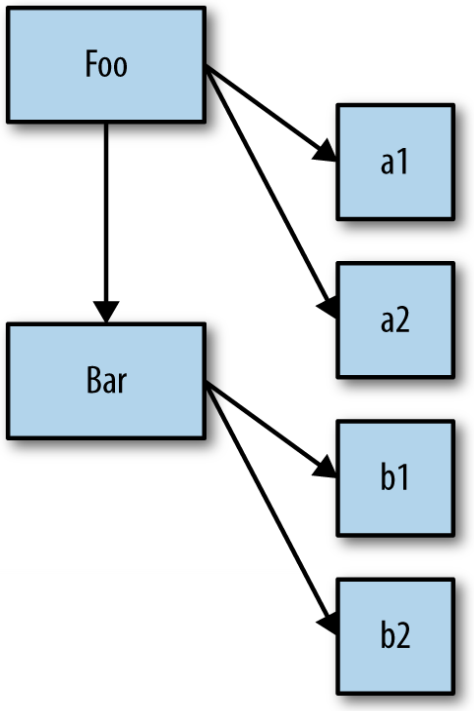
\includegraphics[width=0.3\textwidth]{images/classes_Simpson_p70.png}
	\caption{\label{classes}Vererbungshierarchie in einer klassischen OO-Sprache \\(aus \citep[p. 70]{SimpsonThisobjectprototypes2014}).}
\end{figure}

In Abbildung \ref{classes} ist eine solche (einfache) Hierarchie dargestellt. Ausgehend von der Klassendefinition \texttt{Foo} werden die beiden Objekte \texttt{a1} und \texttt{a2} instantiiert. Die Klasse \texttt{Bar} erbt alle Eigenschaften von \texttt{Foo} und kann eigene Spezialisierungen hinzufügen. Die konkreten Objekte \texttt{b1} und \texttt{b2} haben alle Fähigkeiten, die auch in der Klassendefinition \texttt{Foo} definiert wurden und haben zusätzlich noch weitere Eigenschaften, die in der Klassendefinition von \texttt{Bar} angegeben sind.

Diese Art der klassischen Objektorientierung ist seit ES6
%\footnote{
%ES6 steht für "`ECMAScript 6"'. \emph{ECMAScript} ist die offizielle Bezeichnung des Sprachstandards "`ECMA-262"', auf dem die als \emph{JavaScript} bezichneten Implementierungen beruhen. Im Folgenden wird weiter von JavaScript gesprochen, wenn allgemein die im Standard "`ECMA-262"' definierte Sprache gemeint ist. Wenn es um eine konkrete Version, oder eine Definition geht, so wird von ES\emph{x} gesprochen, wobei \emph{x} entweder eine Versionsnummer oder eine Jahreszahl ist. Zum Zeitpunkt der Erstellung (Winter 2018) ist  ES9 bzw. ES2018 die letzte Version des verabschiedeten Standards. (siehe \citep{international2018ecmascript})}
durch die Benutzung des Schlüsselwortes \texttt{class} auch in Javascript möglich. Es werden Klassen wie z. B. \texttt{class Foo \{\ldots \}} als Blaupausen definiert. Diese können mittels \texttt{class Bar extends Foo\{\ldots \}} zu klassischen Vererbungshierarchien ausgebaut werden. Damit lässt sich in Javascript sowohl syntaktisch als auch semantisch sehr ähnlich programmieren wie in klassischen OO-Sprachen.

\skippingparagraph

Im Kern ist JavaScript eine prototypenbasierte Programmiersprache, in der Objekte für sich alleine stehen und in der andere Techniken der Code-Wiederverwendung zur Verfügung stehen. Einige anerkannte Mitglieder der Javascript Community sind sogar der Meinung, dass die Einführung klassischer Sprachmittel eher nachteilig ist und damit mehr Probleme einhergehen als gelöst werden. Sie kritisieren die mit \texttt{class} eingeführte klassische Semantik in Javascript zum Teil heftig:

In \citep[p. 48ff. "`Classical Inheritance Is Obsolete"']{ElliottProgrammingJavaScriptapplications2014} führt Eric Elliot als Argumente gegen die klassische Vererbung u. a. an:
\begin{itemize}
	\item "`Tight Coupling"': Vererbung zwischen Klassen ist eine der engsten Kopplungen zwischen Komponenten, die in der Programmierung möglich ist. Die erbende Subklasse muss intime Kenntnisse der Implementierung der Basisklasse haben. Daraus ergibt sich direkt das \emph{Fragile Base Class Problem}, \citep[§6.2]{Steimann.2010}).
	\item "`Inflexible Hierarchies"': Nach einer Weile der Nutzung und bei steigender Benutzerbasis erweisen sich letztendlich sämtliche Klassenhierarchien als falsch, um bestimmte neue Nutzungsfälle damit zu modellieren. Durch die enge Kopplung ist es aber extrem schwierig bis unmöglich, diese Fehler durch Refactoring zu beheben.
	\item "`Gorilla/Banana Problem"': Die Vererbung läuft nach dem "`Alles oder Nichts"'-Prinzip und es ist nicht möglich nur einzelne Eigenschaften einer Basisklasse zu erben. Elliot zitiert \citep{SeibelCodersworkreflections2009}: \begin{quote}
	The problem with object-oriented languages is they’ve got all this implicit environment
	that they carry around with them. You wanted a banana but what you got was a gorilla
	holding the banana and the entire jungle.
	\end{quote}
	\item "`Duplicating by necessity"': Aufgrund der angesprochenen Probleme der klassischen Vererbung kommt es in vielen Applikationen dazu, dass entgegen aller Design-Prinzipien, Code Wiederverwendung durch Copy/Paste geschieht und damit der Idee der Vererbung zuwider läuft. 
\end{itemize}

Auch Douglas Crockford, Autor des Standardwerks "`JavaScript: the good parts"' (\citep{CrockfordJavaScriptgoodparts2008}) spricht sich letztendlich gegen klassische Vererbung in Javascript aus: \begin{quote}
I have been writing JavaScript for 14 years now, and I have never once found need to use an uber function. The super idea is fairly important in the classical pattern, but it appears to be unnecessary in the prototypal and functional patterns. I now see my early attempts to support the classical model in JavaScript as a mistake. \citep{CrockfordClassicalInheritanceJavaScript}
\end{quote}


Als letzter prominenten Vertreter der Kritiker sei hier noch Kyle Simpson erwähnt, der über die mit ES6-eingeführten Klassen in Javascript sagt:
\begin{quote}
Bottom line: if the ES6 \texttt{class} makes it harder to robustly leverage 
\texttt{[[Prototype]]}, and hides the most important nature of the JS object 
mechanism --the live delegation links between objects-- shouldn’t we 
see class as creating more troubles than it solves, and just relegate it
to an antipattern? \citep[p. 153]{SimpsonThisobjectprototypes2014}
\end{quote}

\skippingparagraph
Entsprechend dieser kritischen Einschätzung wurde in dieser Arbeit \emph{nicht} weiter auf die Möglichkeiten eingegangen, Javascript wie eine klassische OO-Sprache zu benutzen. 
%Die weiteren Betrachtungen konzentieren sich vielmehr darauf, was Javascript anders macht als klassische OO-Sprachen, und wie sich Javascript dadurch als einen Vertreter der prototypbasierten OO-Sprachen auszeichnet. 
Obwohl die mit ES6 eingeführten Klassen viele interessante Eigenschaften haben, ist es wichtig, Javascript zuerst als prototypenbasierte Sprache zu verstehen. Erst dann kann fundiert entschieden werden, welches Sprachmittel gewinnbringend eingesetzt werden soll.

Bei der für viele, aus anderen klassischen Sprachen kommende, Entwicklerinnen verlockenden Möglichkeit, über den ES6 \texttt{class}-Mechanismus auch JavaScript wie eine klassische Sprache zu benutzen, wird viel Potential verschwendet, das in der prototypischen und damit flexibleren Objektorientierung von JavaScript liegt.

Aus meiner Sicht ist es daher wichtig, vom prototypischen Ursprung von JavaScript aus zu denken und erst dann, wenn das nicht mehr ausreicht, die Erweiterungen zu betrachten, die der Sprache ein klassisches Gewand überstreifen. Andernfalls besteht die Gefahr, dass mit einen klassischen Hammer in der Hand jedes Problem aussieht wie ein Klassennagel.


\end{document}